% Options for packages loaded elsewhere
\PassOptionsToPackage{unicode}{hyperref}
\PassOptionsToPackage{hyphens}{url}
\PassOptionsToPackage{dvipsnames,svgnames,x11names}{xcolor}
%
\documentclass[
]{article}

\usepackage{amsmath,amssymb}
\usepackage{iftex}
\ifPDFTeX
  \usepackage[T1]{fontenc}
  \usepackage[utf8]{inputenc}
  \usepackage{textcomp} % provide euro and other symbols
\else % if luatex or xetex
  \usepackage{unicode-math}
  \defaultfontfeatures{Scale=MatchLowercase}
  \defaultfontfeatures[\rmfamily]{Ligatures=TeX,Scale=1}
\fi
\usepackage{lmodern}
\ifPDFTeX\else  
    % xetex/luatex font selection
\fi
% Use upquote if available, for straight quotes in verbatim environments
\IfFileExists{upquote.sty}{\usepackage{upquote}}{}
\IfFileExists{microtype.sty}{% use microtype if available
  \usepackage[]{microtype}
  \UseMicrotypeSet[protrusion]{basicmath} % disable protrusion for tt fonts
}{}
\makeatletter
\@ifundefined{KOMAClassName}{% if non-KOMA class
  \IfFileExists{parskip.sty}{%
    \usepackage{parskip}
  }{% else
    \setlength{\parindent}{0pt}
    \setlength{\parskip}{6pt plus 2pt minus 1pt}}
}{% if KOMA class
  \KOMAoptions{parskip=half}}
\makeatother
\usepackage{xcolor}
\usepackage[margin=1in]{geometry}
\setlength{\emergencystretch}{3em} % prevent overfull lines
\setcounter{secnumdepth}{5}
% Make \paragraph and \subparagraph free-standing
\makeatletter
\ifx\paragraph\undefined\else
  \let\oldparagraph\paragraph
  \renewcommand{\paragraph}{
    \@ifstar
      \xxxParagraphStar
      \xxxParagraphNoStar
  }
  \newcommand{\xxxParagraphStar}[1]{\oldparagraph*{#1}\mbox{}}
  \newcommand{\xxxParagraphNoStar}[1]{\oldparagraph{#1}\mbox{}}
\fi
\ifx\subparagraph\undefined\else
  \let\oldsubparagraph\subparagraph
  \renewcommand{\subparagraph}{
    \@ifstar
      \xxxSubParagraphStar
      \xxxSubParagraphNoStar
  }
  \newcommand{\xxxSubParagraphStar}[1]{\oldsubparagraph*{#1}\mbox{}}
  \newcommand{\xxxSubParagraphNoStar}[1]{\oldsubparagraph{#1}\mbox{}}
\fi
\makeatother


\providecommand{\tightlist}{%
  \setlength{\itemsep}{0pt}\setlength{\parskip}{0pt}}\usepackage{longtable,booktabs,array}
\usepackage{calc} % for calculating minipage widths
% Correct order of tables after \paragraph or \subparagraph
\usepackage{etoolbox}
\makeatletter
\patchcmd\longtable{\par}{\if@noskipsec\mbox{}\fi\par}{}{}
\makeatother
% Allow footnotes in longtable head/foot
\IfFileExists{footnotehyper.sty}{\usepackage{footnotehyper}}{\usepackage{footnote}}
\makesavenoteenv{longtable}
\usepackage{graphicx}
\makeatletter
\newsavebox\pandoc@box
\newcommand*\pandocbounded[1]{% scales image to fit in text height/width
  \sbox\pandoc@box{#1}%
  \Gscale@div\@tempa{\textheight}{\dimexpr\ht\pandoc@box+\dp\pandoc@box\relax}%
  \Gscale@div\@tempb{\linewidth}{\wd\pandoc@box}%
  \ifdim\@tempb\p@<\@tempa\p@\let\@tempa\@tempb\fi% select the smaller of both
  \ifdim\@tempa\p@<\p@\scalebox{\@tempa}{\usebox\pandoc@box}%
  \else\usebox{\pandoc@box}%
  \fi%
}
% Set default figure placement to htbp
\def\fps@figure{htbp}
\makeatother

\usepackage{float}
\floatplacement{figure}{H}
\usepackage{booktabs}
\usepackage{colortbl}
\usepackage[table]{xcolor}
\definecolor{light-gray}{gray}{0.9}
\renewcommand{\arraystretch}{1.2}
\let\oldtabular\tabular
\let\oldendtabular\endtabular
\renewenvironment{tabular}{\small\oldtabular}{\oldendtabular}
\setlength{\tabcolsep}{4pt}
\makeatletter
\@ifpackageloaded{caption}{}{\usepackage{caption}}
\AtBeginDocument{%
\ifdefined\contentsname
  \renewcommand*\contentsname{Table of contents}
\else
  \newcommand\contentsname{Table of contents}
\fi
\ifdefined\listfigurename
  \renewcommand*\listfigurename{List of Figures}
\else
  \newcommand\listfigurename{List of Figures}
\fi
\ifdefined\listtablename
  \renewcommand*\listtablename{List of Tables}
\else
  \newcommand\listtablename{List of Tables}
\fi
\ifdefined\figurename
  \renewcommand*\figurename{Figure}
\else
  \newcommand\figurename{Figure}
\fi
\ifdefined\tablename
  \renewcommand*\tablename{Table}
\else
  \newcommand\tablename{Table}
\fi
}
\@ifpackageloaded{float}{}{\usepackage{float}}
\floatstyle{ruled}
\@ifundefined{c@chapter}{\newfloat{codelisting}{h}{lop}}{\newfloat{codelisting}{h}{lop}[chapter]}
\floatname{codelisting}{Listing}
\newcommand*\listoflistings{\listof{codelisting}{List of Listings}}
\makeatother
\makeatletter
\makeatother
\makeatletter
\@ifpackageloaded{caption}{}{\usepackage{caption}}
\@ifpackageloaded{subcaption}{}{\usepackage{subcaption}}
\makeatother

\usepackage[]{biblatex}
\usepackage{bookmark}

\IfFileExists{xurl.sty}{\usepackage{xurl}}{} % add URL line breaks if available
\urlstyle{same} % disable monospaced font for URLs
\hypersetup{
  pdftitle={Supplementary material for: The Drastic Effect of Choice of Spacer-to-Protospacer Search or Alignment Tool in CRISPR-Based Viral Defense Analysis},
  pdfauthor={Uri Neri; Antonio Pedro Camargo; Brian Bushnell; Simon Roux},
  colorlinks=true,
  linkcolor={blue},
  filecolor={Maroon},
  citecolor={Blue},
  urlcolor={Blue},
  pdfcreator={LaTeX via pandoc}}


\title{Supplementary material for: The Drastic Effect of Choice of
Spacer-to-Protospacer Search or Alignment Tool in CRISPR-Based Viral
Defense Analysis}
\author{Uri Neri \and Antonio Pedro Camargo \and Brian
Bushnell \and Simon Roux}
\date{}

\begin{document}
\maketitle


\section{Supplementary Materials}\label{supplementary-materials}

\subsection{Tables}\label{tables}

\subsubsection{1. Tool Configuration
Details}\label{tool-configuration-details}

For full version and build information see the git repo at
\href{https://code.jgi.doe.gov/spacersdb/spacer_matching_bench}{code.jgi.doe.gov/spacersdb/spacer\_matching\_bench}

\begin{longtable}[]{@{}
  >{\raggedright\arraybackslash}p{(\linewidth - 4\tabcolsep) * \real{0.0245}}
  >{\raggedright\arraybackslash}p{(\linewidth - 4\tabcolsep) * \real{0.0502}}
  >{\raggedright\arraybackslash}p{(\linewidth - 4\tabcolsep) * \real{0.9252}}@{}}
\toprule\noalign{}
\begin{minipage}[b]{\linewidth}\raggedright
Tool
\end{minipage} & \begin{minipage}[b]{\linewidth}\raggedright
Version
\end{minipage} & \begin{minipage}[b]{\linewidth}\raggedright
Command
\end{minipage} \\
\midrule\noalign{}
\endhead
\bottomrule\noalign{}
\endlastfoot
bbmapskimmer & 39.13 &
\texttt{bbmapskimmer.sh\ sam=1.4\ maxindel=0\ tipsearch=0\ midpad=100\ in=\{spacers\_file\}\ ref=./\{contigs\_file\}\ outm=\{output\_dir\}/bbmap\_skimmer\_output.sam\ t=\{threads\}\ minid=0.85\ path=\{output\_dir\}} \\
blastn & 2.16.0+, Dec 14 2024 &
\texttt{makeblastdb\ -in\ \{contigs\_file\}\ -dbtype\ nucl\ -out\ \{output\_dir\}/contigs\_blastdb\textasciigrave{}\textasciigrave{}blastn\ -query\ \{spacers\_file\}\ -db\ \{output\_dir\}/contigs\_blastdb\ -max\_target\_seqs\ 1000000\ -out\ \{output\_dir\}/blastn\_output.tsv\ -evalue\ 1e-5\ -num\_threads\ \{threads\}\ -task\ blastn-short\ -outfmt\ 6\ qaccver\ saccver\ nident\ length\ mismatch\ qlen\ gapopen\ qstart\ qend\ sstart\ send\ evalue\ bitscore""} \\
bowtie1 & bowtie-align-s version 1.3.1 &
\texttt{bowtie-build\ -\/-threads\ \{threads\}\ \{contigs\_file\}\ \{results\_dir\}/simulated\_data/bt1\_contigs\_index\textasciigrave{}\textasciigrave{}bowtie\ -\/-threads\ \{threads\}\ -f\ -\/-all\ -v\ 3\ -x\ \{results\_dir\}/simulated\_data/bt1\_contigs\_index\ \{spacers\_file\}\ -S\ \{output\_dir\}/bowtie1\_output.sam} \\
bowtie2 & bowtie2-align-s 2.5.4 &
\texttt{bowtie2-build\ -\/-large-index\ -\/-threads\ \{threads\}\ \{contigs\_file\}\ \{results\_dir\}/simulated\_data/contigs\_bt2indx\textasciigrave{}\textasciigrave{}bowtie2\ -\/-all\ -\/-xeq\ -\/-very-sensitive\ -x\ \{results\_dir\}/simulated\_data/contigs\_bt2indx\ -f\ \{spacers\_file\}\ -S\ \{output\_dir\}/bowtie2\_output.sam\ -\/-threads\ \{threads\}} \\
hisat2 & hisat2-align-s 2.2.1 &
\texttt{hisat2-build\ -p\ \{threads\}\ \{contigs\_file\}\ \{output\_dir\}/hisat2\_idx\textasciigrave{}\textasciigrave{}hisat2\ -a\ -\/-no-spliced-alignment\ -\/-no-unal\ -\/-no-softclip\ -\/-secondary\ -p\ \{threads\}\ -x\ \{output\_dir\}/hisat2\_idx\ -f\ \{spacers\_file\}\ -S\ \{output\_dir\}/hisat2\_output.sam} \\
lexicmap & v0.5.0 (06741c8) &
\texttt{mkdir\ -p\ \{output\_dir\}/tmp\_lexicmap\_contigs\ \{output\_dir\}/tmp\_lexicmap\_spacers\textasciigrave{}\textasciigrave{}cp\ \{contigs\_file\}\ \{output\_dir\}/tmp\_lexicmap\_contigs/simulated\_contigs.fa\textasciigrave{}\textasciigrave{}cp\ \{spacers\_file\}\ \{output\_dir\}/tmp\_lexicmap\_spacers/simulated\_spacers.fa\textasciigrave{}\textasciigrave{}lexicmap\ index\ -k\ 15\ -m\ 40000\ -\/-seed-max-desert\ 200\ -\/-seed-in-desert-dist\ 50\ -I\ \{output\_dir\}/tmp\_lexicmap\_contigs\ -O\ \{output\_dir\}/tmp\_lexicmap.lmi\textasciigrave{}\textasciigrave{}lexicmap\ search\ -d\ \{output\_dir\}/tmp\_lexicmap.lmi\ \{output\_dir\}/tmp\_lexicmap\_spacers/simulated\_spacers.fa\ -o\ \{output\_dir\}/lexicmap\_output.tsv\ -\/-threads\ \{threads\}\ -\/-align-min-match-len\ 17\ -\/-align-min-match-pident\ 85\ -\/-seed-min-prefix\ 15\ -\/-seed-min-single-prefix\ 15\ -\/-seed-max-dist\ 100\ -\/-seed-max-gap\ 100\ -\/-align-max-gap\ 20\ -\/-align-band\ 100\ -\/-top-n-genomes\ 0\ -a} \\
minimap2 & 2.28-r1209 &
\texttt{minimap2\ -N\ 100\ -\/-eqx\ -t\ \{threads\}\ -a\ \{contigs\_file\}\ \{spacers\_file\}\ -o\ \{output\_dir\}/minimap2\_output.sam} \\
mmseqs2 & db8ad2d14d0a285ce0ad62bbefd0dce927663315 &
\texttt{mkdir\ -p\ \{output\_dir\}/tmp\_spacers\ \{output\_dir\}/tmp\_contigs\ \{output\_dir\}/tmp\_mmseqs\ \{output\_dir\}/tmp\_mmseqs\_outputs\textasciigrave{}\textasciigrave{}mmseqs\ createdb\ \{spacers\_file\}\ \{output\_dir\}/tmp\_spacers/mmdb\textasciigrave{}\textasciigrave{}mmseqs\ createdb\ \{contigs\_file\}\ \{output\_dir\}/tmp\_contigs/mmdb\textasciigrave{}\textasciigrave{}mmseqs\ search\ \{output\_dir\}/tmp\_spacers/mmdb\ \{output\_dir\}/tmp\_contigs/mmdb\ \{output\_dir\}/tmp\_mmseqs\_outputs/mmseqs\_output\ \{output\_dir\}/tmp\_mmseqs\ -\/-min-seq-id\ 0.85\ -\/-min-aln-len\ 17\ -\/-threads\ \{threads\}\ -a\ -\/-search-type\ 3\ -v\ 1\textasciigrave{}\textasciigrave{}mmseqs\ convertalis\ \{output\_dir\}/tmp\_spacers/mmdb\ \{output\_dir\}/tmp\_contigs/mmdb\ \{output\_dir\}/tmp\_mmseqs\_outputs/mmseqs\_output\ \{output\_dir\}/mmseqs\_output.tsv\ -\/-format-mode\ 0\ -\/-search-type\ 4\ -\/-format-output\ query,target,nident,alnlen,mismatch,qlen,gapopen,qstart,qend,tstart,tend,evalue,bits} \\
mummer4 & 4.1.0-r1304 // 4.1 &
\texttt{nucmer\ -\/-maxmatch\ -\/-nosimplify\ -\/-batch=10000000\ -\/-threads\ \{threads\}\ -\/-sam-long=\{output\_dir\}/mummer4\_output.sam\ -c\ 1\ \{contigs\_file\}\ \{spacers\_file\}} \\
spacer\_containment & 0.1.0 &
\texttt{spacer-containment\ -\/-n-threads\ \{threads\}\ \{contigs\_file\}\ \{spacers\_file\}\ \textgreater{}\ \{output\_dir\}/spacer\_containment\_output.tsv} \\
strobealign & 0.15.0 &
\texttt{strobealign\ -\/-eqx\ -k\ 15\ -N\ 1000\ -t\ \{threads\}\ \{contigs\_file\}\ \{spacers\_file\}\ -o\ \{output\_dir\}/strobealign\_output.sam} \\
\end{longtable}

\subsubsection{2. Recall values for each tool at different mismatch
thresholds}\label{recall-values-for-each-tool-at-different-mismatch-thresholds}

\paragraph{A. IMG/VR4 dataset}\label{a.-imgvr4-dataset}

Every row lists the results for a specific mismatch threshold and
tool.\\
The values are for exact mismatches (not max), and represent the total
number of unique spacer-contig pairs (aligning at that mismatch
threshold).\\
The fraction is tool\_matches divided by total\_possible.

\begin{longtable}[]{@{}
  >{\raggedright\arraybackslash}p{(\linewidth - 8\tabcolsep) * \real{0.1644}}
  >{\raggedright\arraybackslash}p{(\linewidth - 8\tabcolsep) * \real{0.2055}}
  >{\raggedright\arraybackslash}p{(\linewidth - 8\tabcolsep) * \real{0.2192}}
  >{\raggedright\arraybackslash}p{(\linewidth - 8\tabcolsep) * \real{0.1918}}
  >{\raggedright\arraybackslash}p{(\linewidth - 8\tabcolsep) * \real{0.2192}}@{}}
\toprule\noalign{}
\begin{minipage}[b]{\linewidth}\raggedright
mismatches
\end{minipage} & \begin{minipage}[b]{\linewidth}\raggedright
tool
\end{minipage} & \begin{minipage}[b]{\linewidth}\raggedright
total\_possible
\end{minipage} & \begin{minipage}[b]{\linewidth}\raggedright
tool\_matches
\end{minipage} & \begin{minipage}[b]{\linewidth}\raggedright
fraction
\end{minipage} \\
\midrule\noalign{}
\endhead
\bottomrule\noalign{}
\endlastfoot
0 & mummer4 & 16866829 & 16866546 & 0.9999832 \\
0 & mmseqs2 & 16866829 & 15803286 & 0.9369447 \\
0 & bowtie1 & 16866829 & 16866784 & 0.9999973 \\
0 & lexicmap & 16866829 & 6033115 & 0.3576911 \\
0 & minimap2 & 16866829 & 5110 & 0.000303 \\
0 & strobealign & 16866829 & 4233236 & 0.25098 \\
0 & blastn & 16866829 & 16850968 & 0.9990596 \\
0 & bbmap\_skimmer & 16866829 & 14978104 & 0.8880213 \\
0 & bowtie2 & 16866829 & 16866667 & 0.9999904 \\
1 & mummer4 & 12197007 & 8032640 & 0.6585747 \\
1 & mmseqs2 & 12197007 & 9805301 & 0.8039104 \\
1 & bowtie1 & 12197007 & 11992384 & 0.9832235 \\
1 & lexicmap & 12197007 & 835330 & 0.0684865 \\
1 & minimap2 & 12197007 & 1086 & 0.000089038237 \\
1 & strobealign & 12197007 & 1311189 & 0.1075009 \\
1 & blastn & 12197007 & 7318398 & 0.6000159 \\
1 & bbmap\_skimmer & 12197007 & 2413864 & 0.1979063 \\
1 & bowtie2 & 12197007 & 12112313 & 0.9930562 \\
2 & mummer4 & 12359867 & 3129926 & 0.253233 \\
2 & mmseqs2 & 12359867 & 6756086 & 0.5466148 \\
2 & bowtie1 & 12359867 & 11173197 & 0.9039901 \\
2 & lexicmap & 12359867 & 426554 & 0.0345112 \\
2 & minimap2 & 12359867 & 667 & 0.000053964982 \\
2 & strobealign & 12359867 & 375251 & 0.0303604 \\
2 & blastn & 12359867 & 3217012 & 0.2602789 \\
2 & bbmap\_skimmer & 12359867 & 1047205 & 0.0847262 \\
2 & bowtie2 & 12359867 & 5243454 & 0.4242322 \\
3 & mummer4 & 16472212 & 673444 & 0.0408836 \\
3 & mmseqs2 & 16472212 & 3560155 & 0.216131 \\
3 & bowtie1 & 16472212 & 14523177 & 0.8816774 \\
3 & lexicmap & 16472212 & 430208 & 0.0261172 \\
3 & minimap2 & 16472212 & 392 & 0.000023797654 \\
3 & strobealign & 16472212 & 88246 & 0.0053573 \\
3 & blastn & 16472212 & 1972148 & 0.1197258 \\
3 & bbmap\_skimmer & 16472212 & 630914 & 0.0383017 \\
3 & bowtie2 & 16472212 & 2998722 & 0.1820473 \\
\end{longtable}

\paragraph{B. Synthetic dataset}\label{b.-synthetic-dataset}

\begin{longtable}[]{@{}
  >{\raggedright\arraybackslash}p{(\linewidth - 16\tabcolsep) * \real{0.0822}}
  >{\raggedright\arraybackslash}p{(\linewidth - 16\tabcolsep) * \real{0.1370}}
  >{\raggedright\arraybackslash}p{(\linewidth - 16\tabcolsep) * \real{0.1096}}
  >{\raggedright\arraybackslash}p{(\linewidth - 16\tabcolsep) * \real{0.0959}}
  >{\raggedright\arraybackslash}p{(\linewidth - 16\tabcolsep) * \real{0.1233}}
  >{\raggedright\arraybackslash}p{(\linewidth - 16\tabcolsep) * \real{0.1164}}
  >{\raggedright\arraybackslash}p{(\linewidth - 16\tabcolsep) * \real{0.1164}}
  >{\raggedright\arraybackslash}p{(\linewidth - 16\tabcolsep) * \real{0.0959}}
  >{\raggedright\arraybackslash}p{(\linewidth - 16\tabcolsep) * \real{0.1233}}@{}}
\toprule\noalign{}
\begin{minipage}[b]{\linewidth}\raggedright
mismatches
\end{minipage} & \begin{minipage}[b]{\linewidth}\raggedright
tool
\end{minipage} & \begin{minipage}[b]{\linewidth}\raggedright
total\_possible
\end{minipage} & \begin{minipage}[b]{\linewidth}\raggedright
tool\_matches
\end{minipage} & \begin{minipage}[b]{\linewidth}\raggedright
recall
\end{minipage} & \begin{minipage}[b]{\linewidth}\raggedright
false\_positives
\end{minipage} & \begin{minipage}[b]{\linewidth}\raggedright
false\_negatives
\end{minipage} & \begin{minipage}[b]{\linewidth}\raggedright
precision
\end{minipage} & \begin{minipage}[b]{\linewidth}\raggedright
f1\_score
\end{minipage} \\
\midrule\noalign{}
\endhead
\bottomrule\noalign{}
\endlastfoot
0 & minimap2 & 1899024 & 176 & 0.00009267918678 & 49 & 1898848 &
0.7822222222 & 0.0001853364146 \\
0 & bbmapskimmer & 1899024 & 377426 & 0.1987473565 & 1010 & 1521598 &
0.9973311207 & 0.3314446796 \\
0 & mmseqs2map & 1899024 & 1021533 & 0.5379252711 & 57809 & 877491 &
0.9464405165 & 0.6859687493 \\
0 & mmseqs2 & 1899024 & 1021533 & 0.5379252711 & 134608 & 877491 &
0.8835712945 & 0.6687252571 \\
0 & minimap2\_mod & 1899024 & 176 & 0.00009267918678 & 49 & 1898848 &
0.7822222222 & 0.0001853364146 \\
0 & bowtie1 & 1899024 & 1899024 & 1 & 0 & 0 & 1 & 1 \\
0 & bbmapskimmermod & 1899024 & 1899024 & 1 & 1130 & 0 & 0.9994053114 &
0.9997025672 \\
0 & bwa\_mem & 1899024 & 683227 & 0.3597779702 & 15626 & 1215797 &
0.9776405052 & 0.5259887208 \\
0 & lexicmap & 1899024 & 1427612 & 0.7517609045 & 469844 & 471412 &
0.7523821369 & 0.7520713924 \\
0 & hisat2 & 1899024 & 1875654 & 0.9876936784 & 3 & 23370 & 0.9999984006
& 0.9938079536 \\
0 & minimap2\_og & 1899024 & 48 & 0.00002527614185 & 6 & 1898976 &
0.8888888889 & 0.00005055084625 \\
0 & spacer\_containment & 1899024 & 1899024 & 1 & 0 & 0 & 1 & 1 \\
0 & bowtie2 & 1899024 & 1899024 & 1 & 3 & 0 & 0.9999984202 &
0.9999992101 \\
0 & blastn & 1899024 & 1745238 & 0.919018401 & 596453 & 153786 &
0.7452896219 & 0.8230866729 \\
0 & mummer4 & 1899024 & 1860393 & 0.9796574451 & 250245 & 38631 &
0.881436324 & 0.9279550246 \\
0 & strobealign & 1899024 & 42016 & 0.0221250495 & 193 & 1857008 &
0.9954275155 & 0.04328795152 \\
1 & minimap2 & 1992339 & 86 & 0.00004316534485 & 49 & 1992253 &
0.637037037 & 0.00008632484037 \\
1 & bbmapskimmer & 1992339 & 814246 & 0.4086884812 & 1010 & 1178093 &
0.9987611253 & 0.5800309518 \\
1 & mmseqs2map & 1992339 & 982267 & 0.4930220209 & 57809 & 1010072 &
0.9444184848 & 0.6478447046 \\
1 & mmseqs2 & 1992339 & 971696 & 0.4877161969 & 134608 & 1020643 &
0.8783263913 & 0.627175186 \\
1 & minimap2\_mod & 1992339 & 86 & 0.00004316534485 & 49 & 1992253 &
0.637037037 & 0.00008632484037 \\
1 & bowtie1 & 1992339 & 1924529 & 0.9659646275 & 0 & 67810 & 1 &
0.9826876984 \\
1 & bbmapskimmermod & 1992339 & 1903036 & 0.9551768048 & 1130 & 89303 &
0.9994065643 & 0.9767912527 \\
1 & bwa\_mem & 1992339 & 569097 & 0.2856426542 & 15626 & 1423242 &
0.9732762351 & 0.4416634136 \\
1 & lexicmap & 1992339 & 848885 & 0.4260745787 & 469844 & 1143454 &
0.643714516 & 0.512756005 \\
1 & hisat2 & 1992339 & 1638156 & 0.8222275426 & 3 & 354183 &
0.9999981687 & 0.9024414832 \\
1 & minimap2\_og & 1992339 & 12 & 0.00000602 & 6 & 1992327 &
0.6666666667 & 0.00001204603392 \\
1 & spacer\_containment & 0 & 0 & 0 & 0 & 0 & 0 & 0 \\
1 & bowtie2 & 1992339 & 1924529 & 0.9659646275 & 3 & 67810 &
0.9999984412 & 0.9826869458 \\
1 & blastn & 1992339 & 1534121 & 0.7700100234 & 596453 & 458218 &
0.7200505591 & 0.7441927589 \\
1 & mummer4 & 1992339 & 1605268 & 0.8057203117 & 250245 & 387071 &
0.8651343321 & 0.8343709685 \\
1 & strobealign & 1992339 & 39698 & 0.01992532395 & 193 & 1952641 &
0.9951618159 & 0.03906841253 \\
2 & minimap2 & 2137067 & 91 & 0.00004258172533 & 49 & 2136976 & 0.65 &
0.00008515787193 \\
2 & bbmapskimmer & 2137067 & 804812 & 0.3765965222 & 1010 & 1332255 &
0.9987466215 & 0.5469536907 \\
2 & mmseqs2map & 2137067 & 912682 & 0.4270722443 & 57809 & 1224385 &
0.9404332446 & 0.5873949899 \\
2 & mmseqs2 & 2137067 & 901193 & 0.4216961845 & 134608 & 1235874 &
0.8700445356 & 0.5680620814 \\
2 & minimap2\_mod & 2137067 & 91 & 0.00004258172533 & 49 & 2136976 &
0.65 & 0.00008515787193 \\
2 & bowtie1 & 2137067 & 1934586 & 0.9052528536 & 0 & 202481 & 1 &
0.9502705658 \\
2 & bbmapskimmermod & 2137067 & 1734297 & 0.811531412 & 1130 & 402770 &
0.9993488634 & 0.8957002903 \\
2 & bwa\_mem & 2137067 & 515856 & 0.2413850385 & 15626 & 1621211 &
0.9705991924 & 0.3866190952 \\
2 & lexicmap & 2137067 & 562385 & 0.2631574022 & 469844 & 1574682 &
0.544825809 & 0.3548958507 \\
2 & hisat2 & 2137067 & 1115625 & 0.5220355749 & 3 & 1021442 &
0.9999973109 & 0.6859696344 \\
2 & minimap2\_og & 2137067 & 26 & 0.00001216620724 & 6 & 2137041 &
0.8125 & 0.00002433205013 \\
2 & spacer\_containment & 0 & 0 & 0 & 0 & 0 & 0 & 0 \\
2 & bowtie2 & 2137067 & 1573821 & 0.7364397092 & 3 & 563246 &
0.9999980938 & 0.8482173149 \\
2 & blastn & 2137067 & 1355458 & 0.6342608819 & 596453 & 781609 &
0.6944261291 & 0.6629813122 \\
2 & mummer4 & 2137067 & 1432751 & 0.6704286763 & 250245 & 704316 &
0.851309807 & 0.7501190425 \\
2 & strobealign & 2137067 & 34729 & 0.01625077735 & 193 & 2102338 &
0.9944733979 & 0.03197898332 \\
3 & minimap2 & 2609997 & 220 & 0.00008429128463 & 49 & 2609777 &
0.8178438662 & 0.000168565196 \\
3 & bbmapskimmer & 2609997 & 760618 & 0.291424856 & 1010 & 1849379 &
0.9986738933 & 0.4511877804 \\
3 & mmseqs2map & 2609997 & 860977 & 0.3298766244 & 57809 & 1749020 &
0.9370811048 & 0.4879738992 \\
3 & mmseqs2 & 2609997 & 862278 & 0.3303750924 & 134608 & 1747719 &
0.8649715213 & 0.4781291769 \\
3 & minimap2\_mod & 2609997 & 228 & 0.00008735642225 & 49 & 2609769 &
0.8231046931 & 0.0001746943041 \\
3 & bowtie1 & 2609997 & 2238309 & 0.8575906409 & 0 & 371688 & 1 &
0.9233365221 \\
3 & bbmapskimmermod & 2609997 & 1534102 & 0.5877792197 & 1130 & 1075895
& 0.9992639549 & 0.7401772013 \\
3 & bwa\_mem & 2609997 & 497712 & 0.1906944721 & 15626 & 2112285 &
0.969560017 & 0.3187054863 \\
3 & lexicmap & 2609997 & 443019 & 0.1697392756 & 469844 & 2166978 &
0.4853072148 & 0.2515109882 \\
3 & hisat2 & 2609997 & 564049 & 0.2161109764 & 3 & 2045948 &
0.9999946813 & 0.3554129127 \\
3 & minimap2\_og & 2609997 & 35 & 0.0000134099771 & 6 & 2609962 &
0.8536585366 & 0.0000268195329 \\
3 & spacer\_containment & 0 & 0 & 0 & 0 & 0 & 0 & 0 \\
3 & bowtie2 & 2609997 & 1415300 & 0.5422611597 & 3 & 1194697 &
0.9999978803 & 0.7032022458 \\
3 & blastn & 2609997 & 1270806 & 0.4868994102 & 596453 & 1339191 &
0.6805729682 & 0.5676718061 \\
3 & mummer4 & 2609997 & 1338301 & 0.5127595932 & 250245 & 1271696 &
0.842469151 & 0.6375073448 \\
3 & strobealign & 2609997 & 30913 & 0.01184407492 & 193 & 2579084 &
0.9937954092 & 0.02340915898 \\
\end{longtable}

\section{Figures}\label{figures}

\subsubsection{Supplementary figure 1.}\label{supplementary-figure-1.}

Benchmarking framework pipeline overview.

\pandocbounded{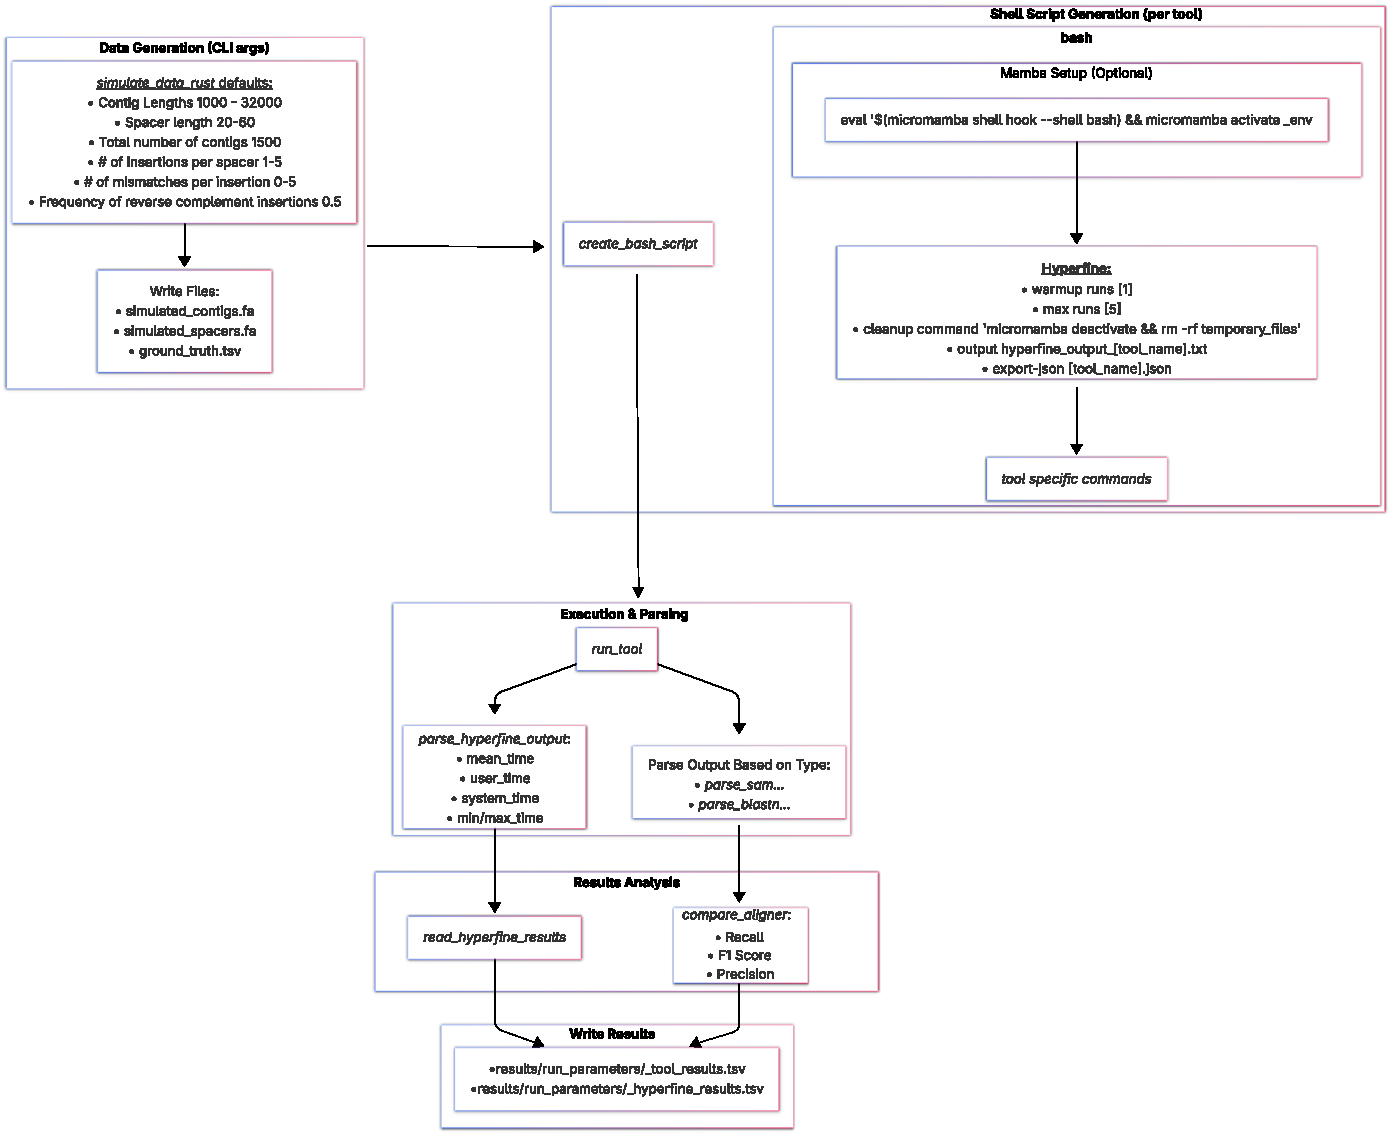
\includegraphics[keepaspectratio]{supplementary_files/mediabag/figures/supp/workflow.pdf}}

\subsubsection{Supplementary figure 2.}\label{supplementary-figure-2.}

IMG/VR v4 based results in a tool vs tool comparison. Unlike the similar
matrix in the main text(figure 1) which showcases the values for up to 1
and 3 mismatches, here the matrixes are separated for each mismatch
threshold at an \textbf{exact} mismatch value. From top left to bottom
right, the mismatch threshold is 0, 1, 2, 3. Like the main text figure,
the value of a cell(i,j) is the fraction of spacer-contig pairs
identified by the tool listed in row i, which were not identified by the
tool listed in the j column.

\pandocbounded{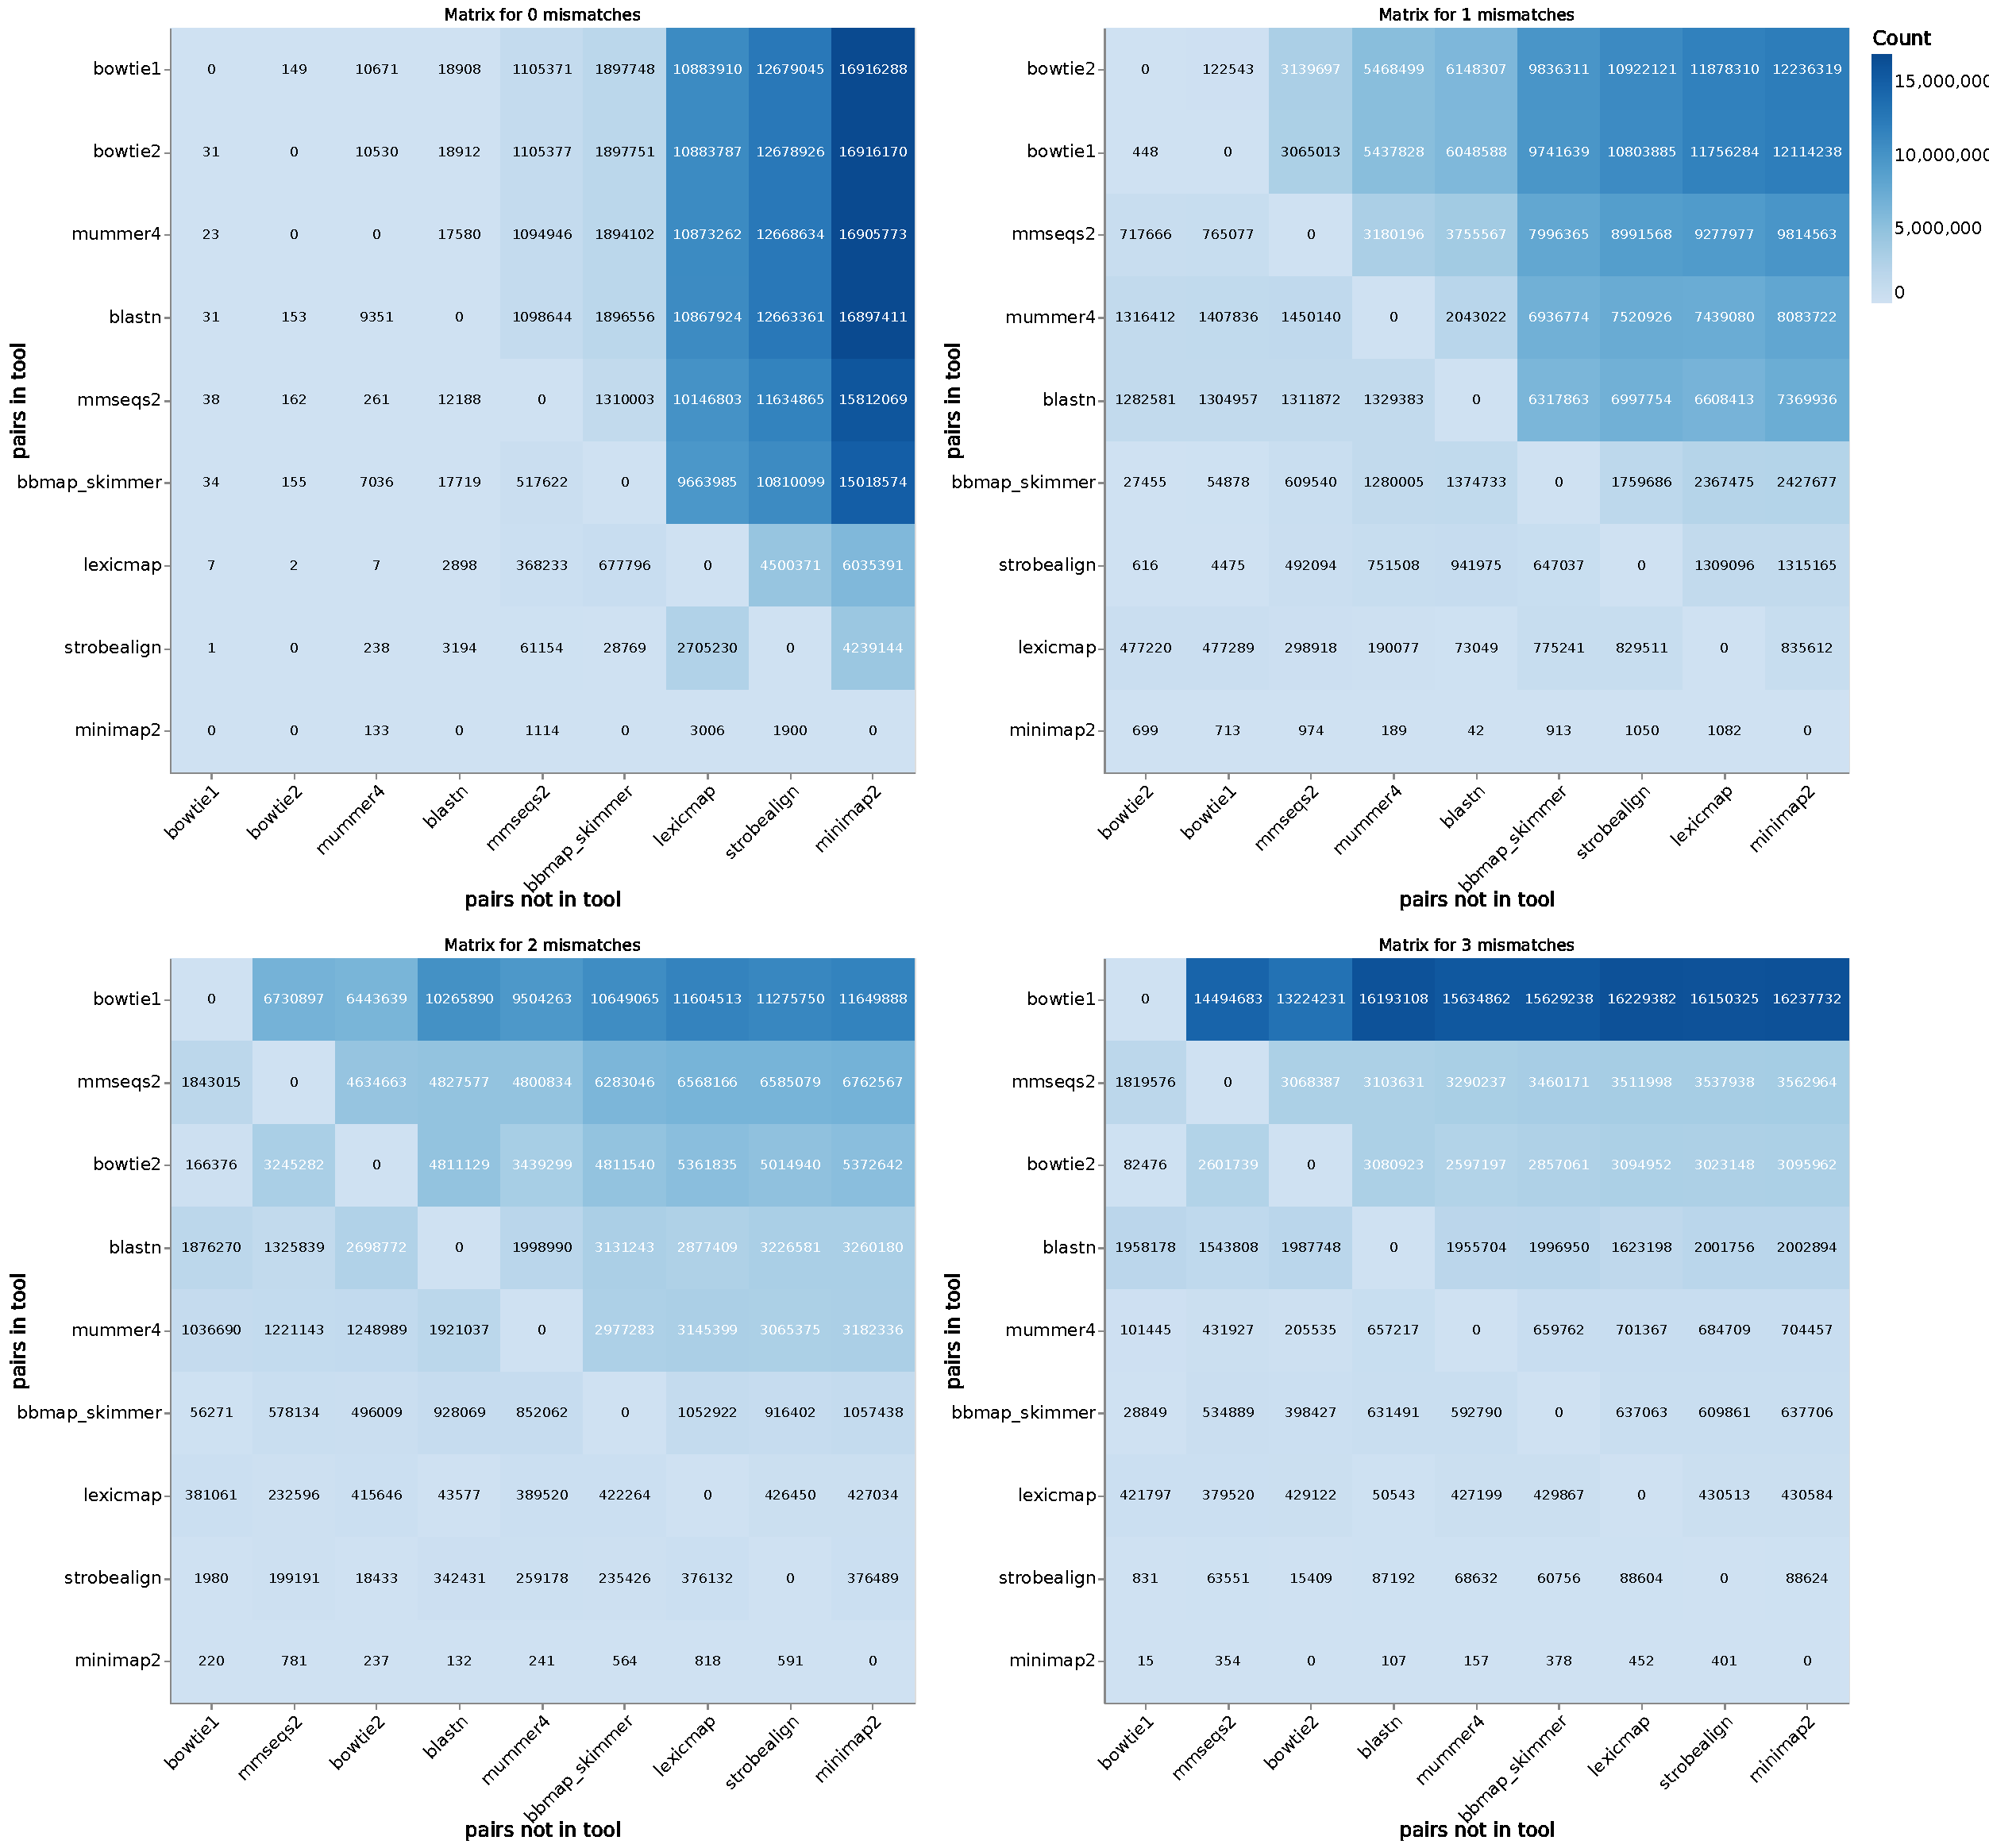
\includegraphics[keepaspectratio]{supplementary_files/mediabag/figures/supp/real_data_matrix_combined.pdf}}

\subsubsection{Supplementary figure 3}\label{supplementary-figure-3}

Simulated dataset performance metrics.\\
Percision = True Positives / (True Positives + False Positives)\\
Recall = True Positives / (True Positives + False Negatives)\\
F1 = 2 * (Percision * Recall) / (Percision + Recall)\\
Note: Because of the various prefiltering steps, the number of False
Negatives and False Positives may not be indicative of the actual raw
tool-reported results. As such, we recommend focusing on the recall rate
between tools, which is equivalent to the fraction of detected
spacer-protospacer pairs out of all the spacer-protospacer pairs in the
reference file.

\pandocbounded{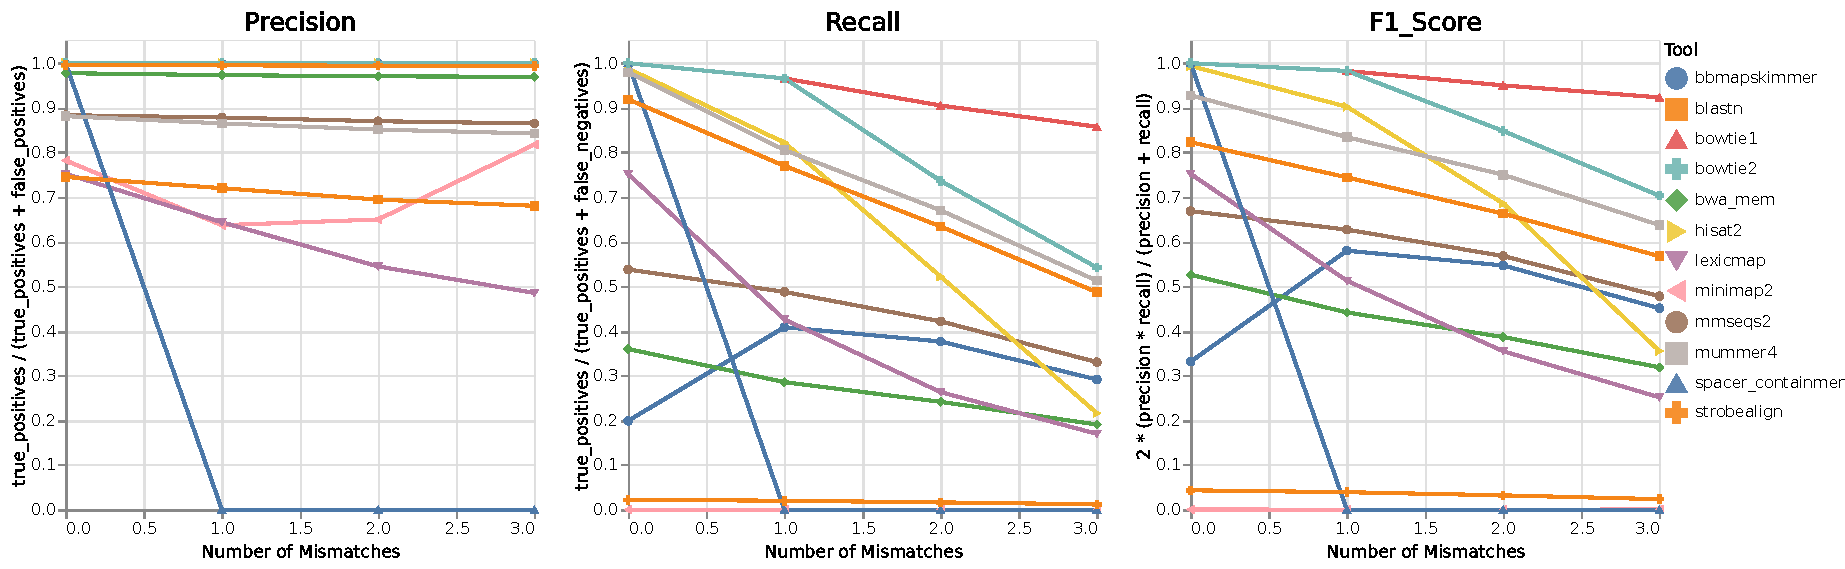
\includegraphics[keepaspectratio]{supplementary_files/mediabag/figures/supp/simulated_tool_performance_by_mismatches.pdf}}

\subsubsection{Supplementary figure 4.}\label{supplementary-figure-4.}

\textbf{Simulated dataset} recall (detection fraction) for different
values of spacer occurrences.

\paragraph{A. for exact mismatches, in a contig dependent
manner}\label{a.-for-exact-mismatches-in-a-contig-dependent-manner}

Per contigs manner means the that the recall measure is the fraction of
occurences each tool identified out of the total number of spacer-contig
pairs, identified by all tools.\\
1. 0 mismatches

\pandocbounded{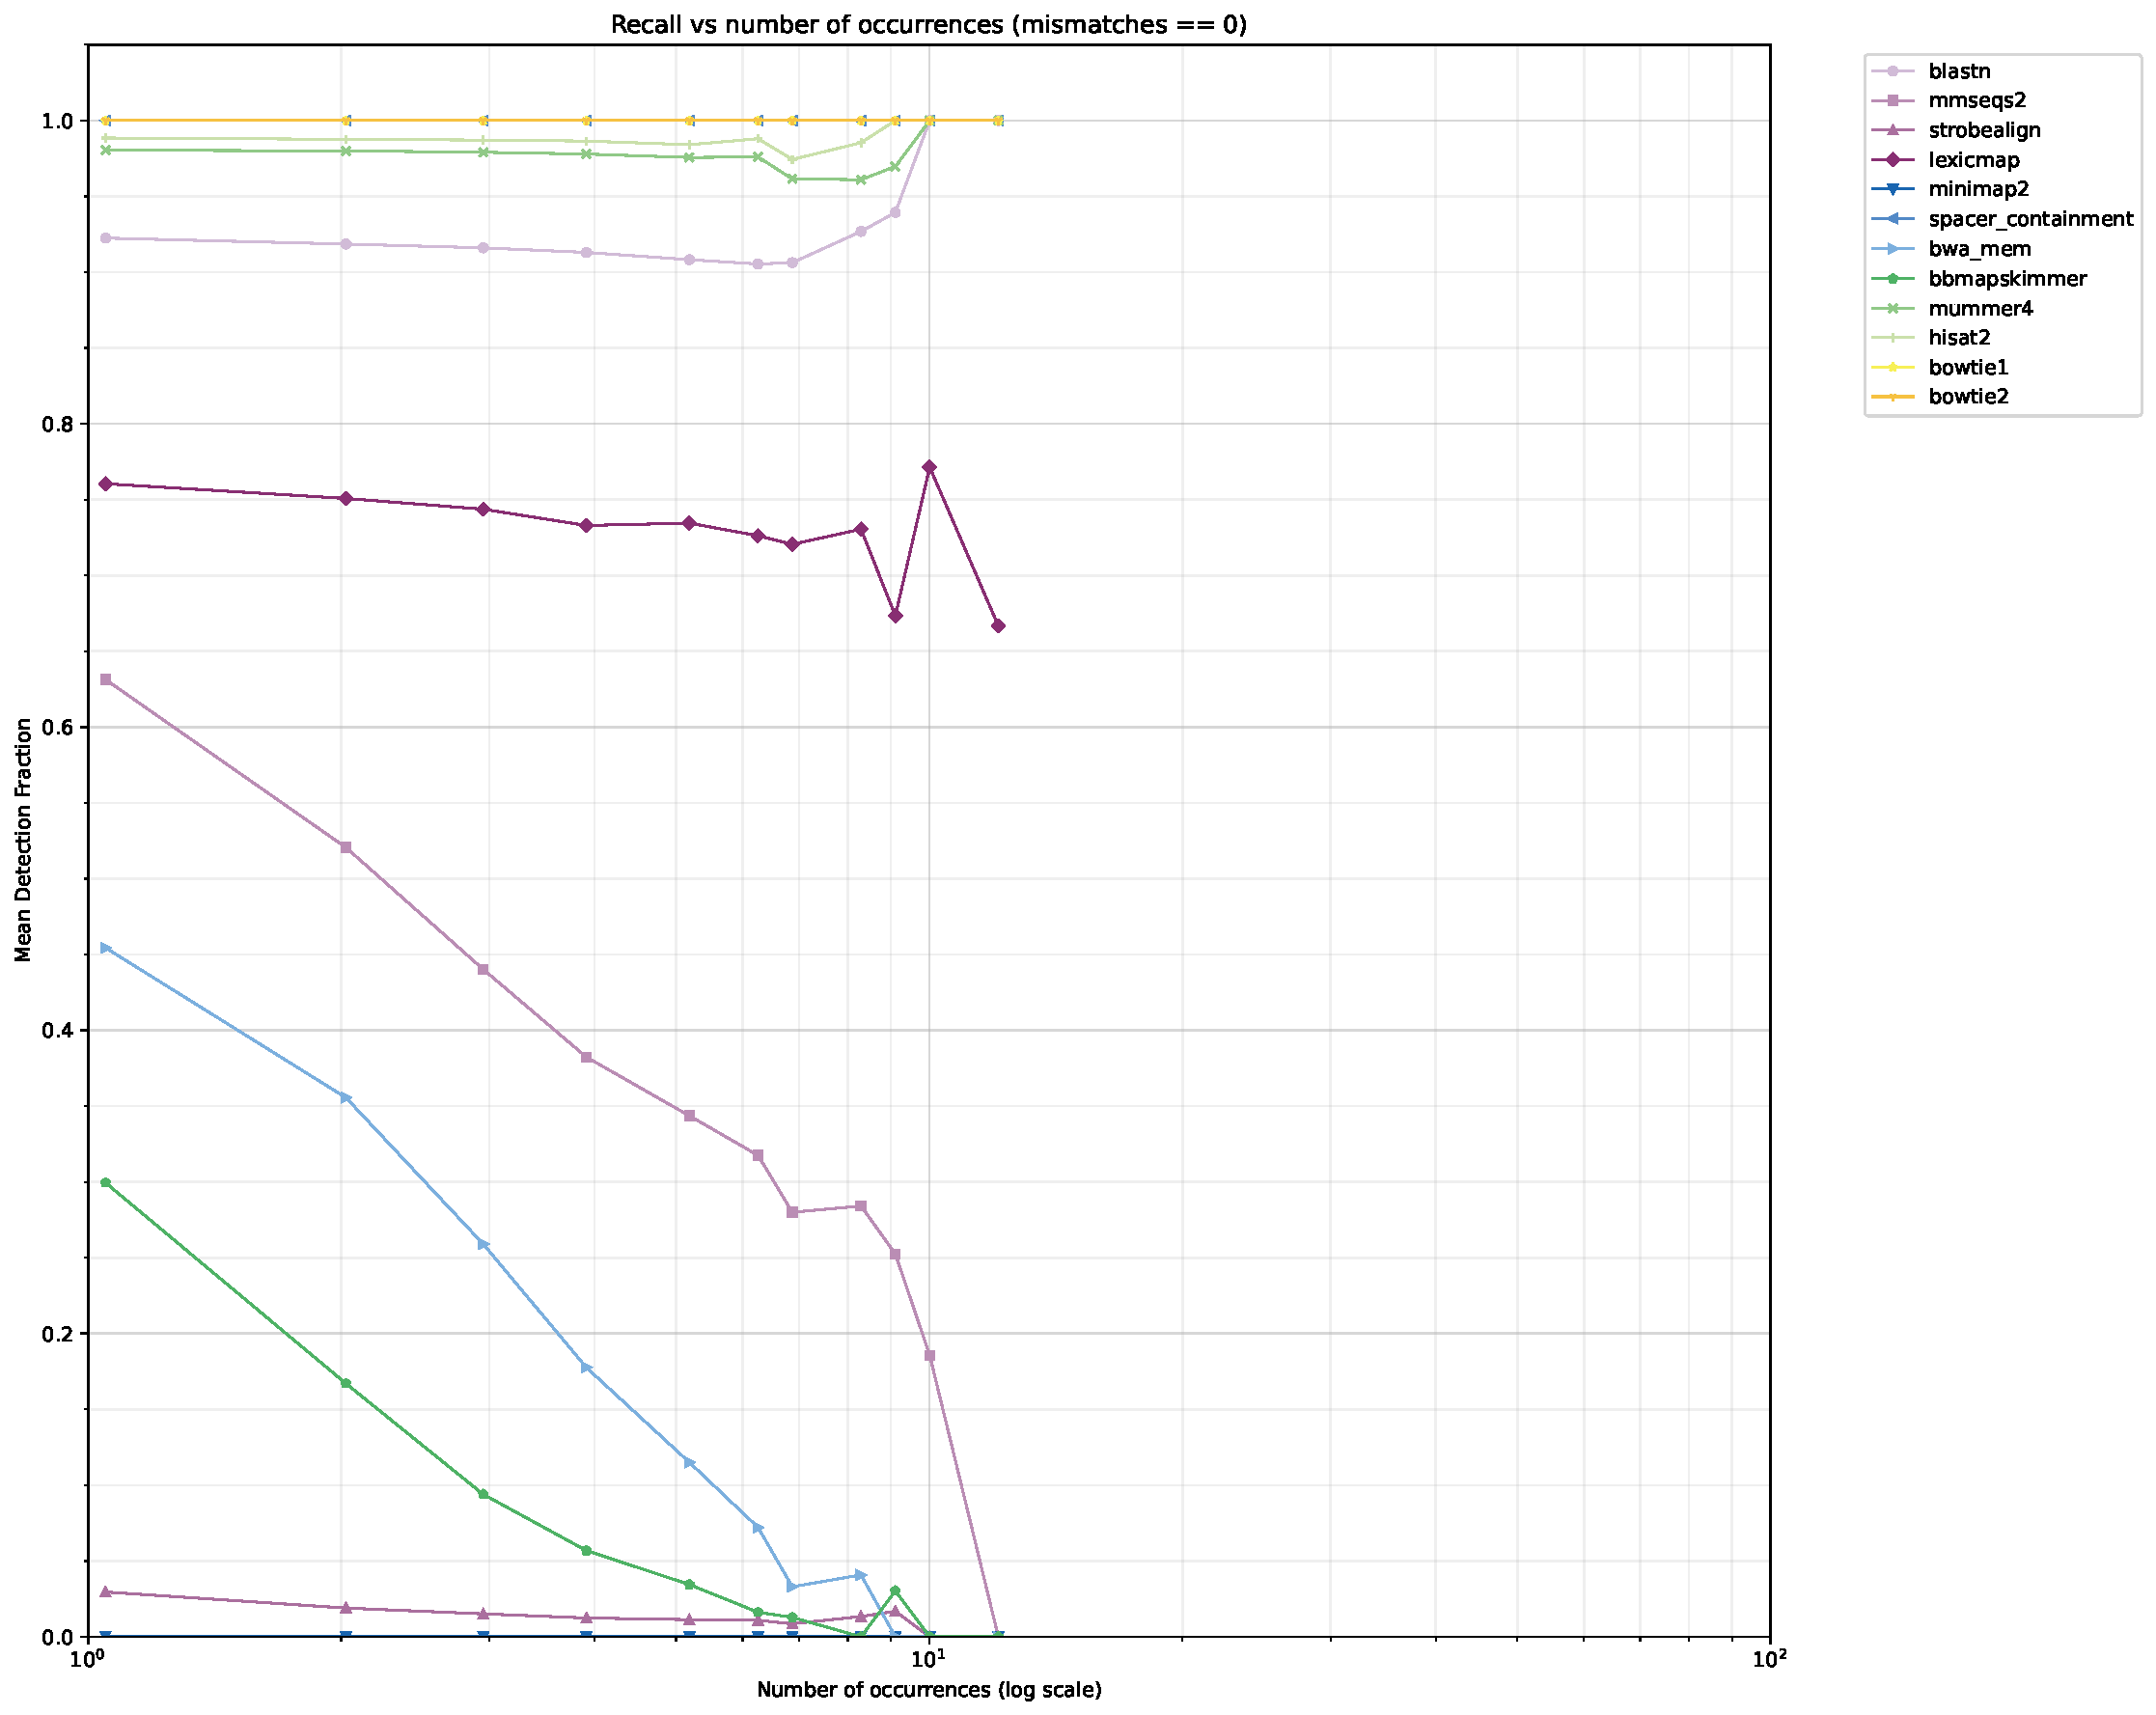
\includegraphics[keepaspectratio]{supplementary_files/mediabag/figures/supp/simulated_recall_vs_occurrences_with_contig_id_exact_nm_0.pdf}}

\begin{enumerate}
\def\labelenumi{\arabic{enumi}.}
\setcounter{enumi}{1}
\tightlist
\item
  exactly 1 mismatch
\end{enumerate}

\pandocbounded{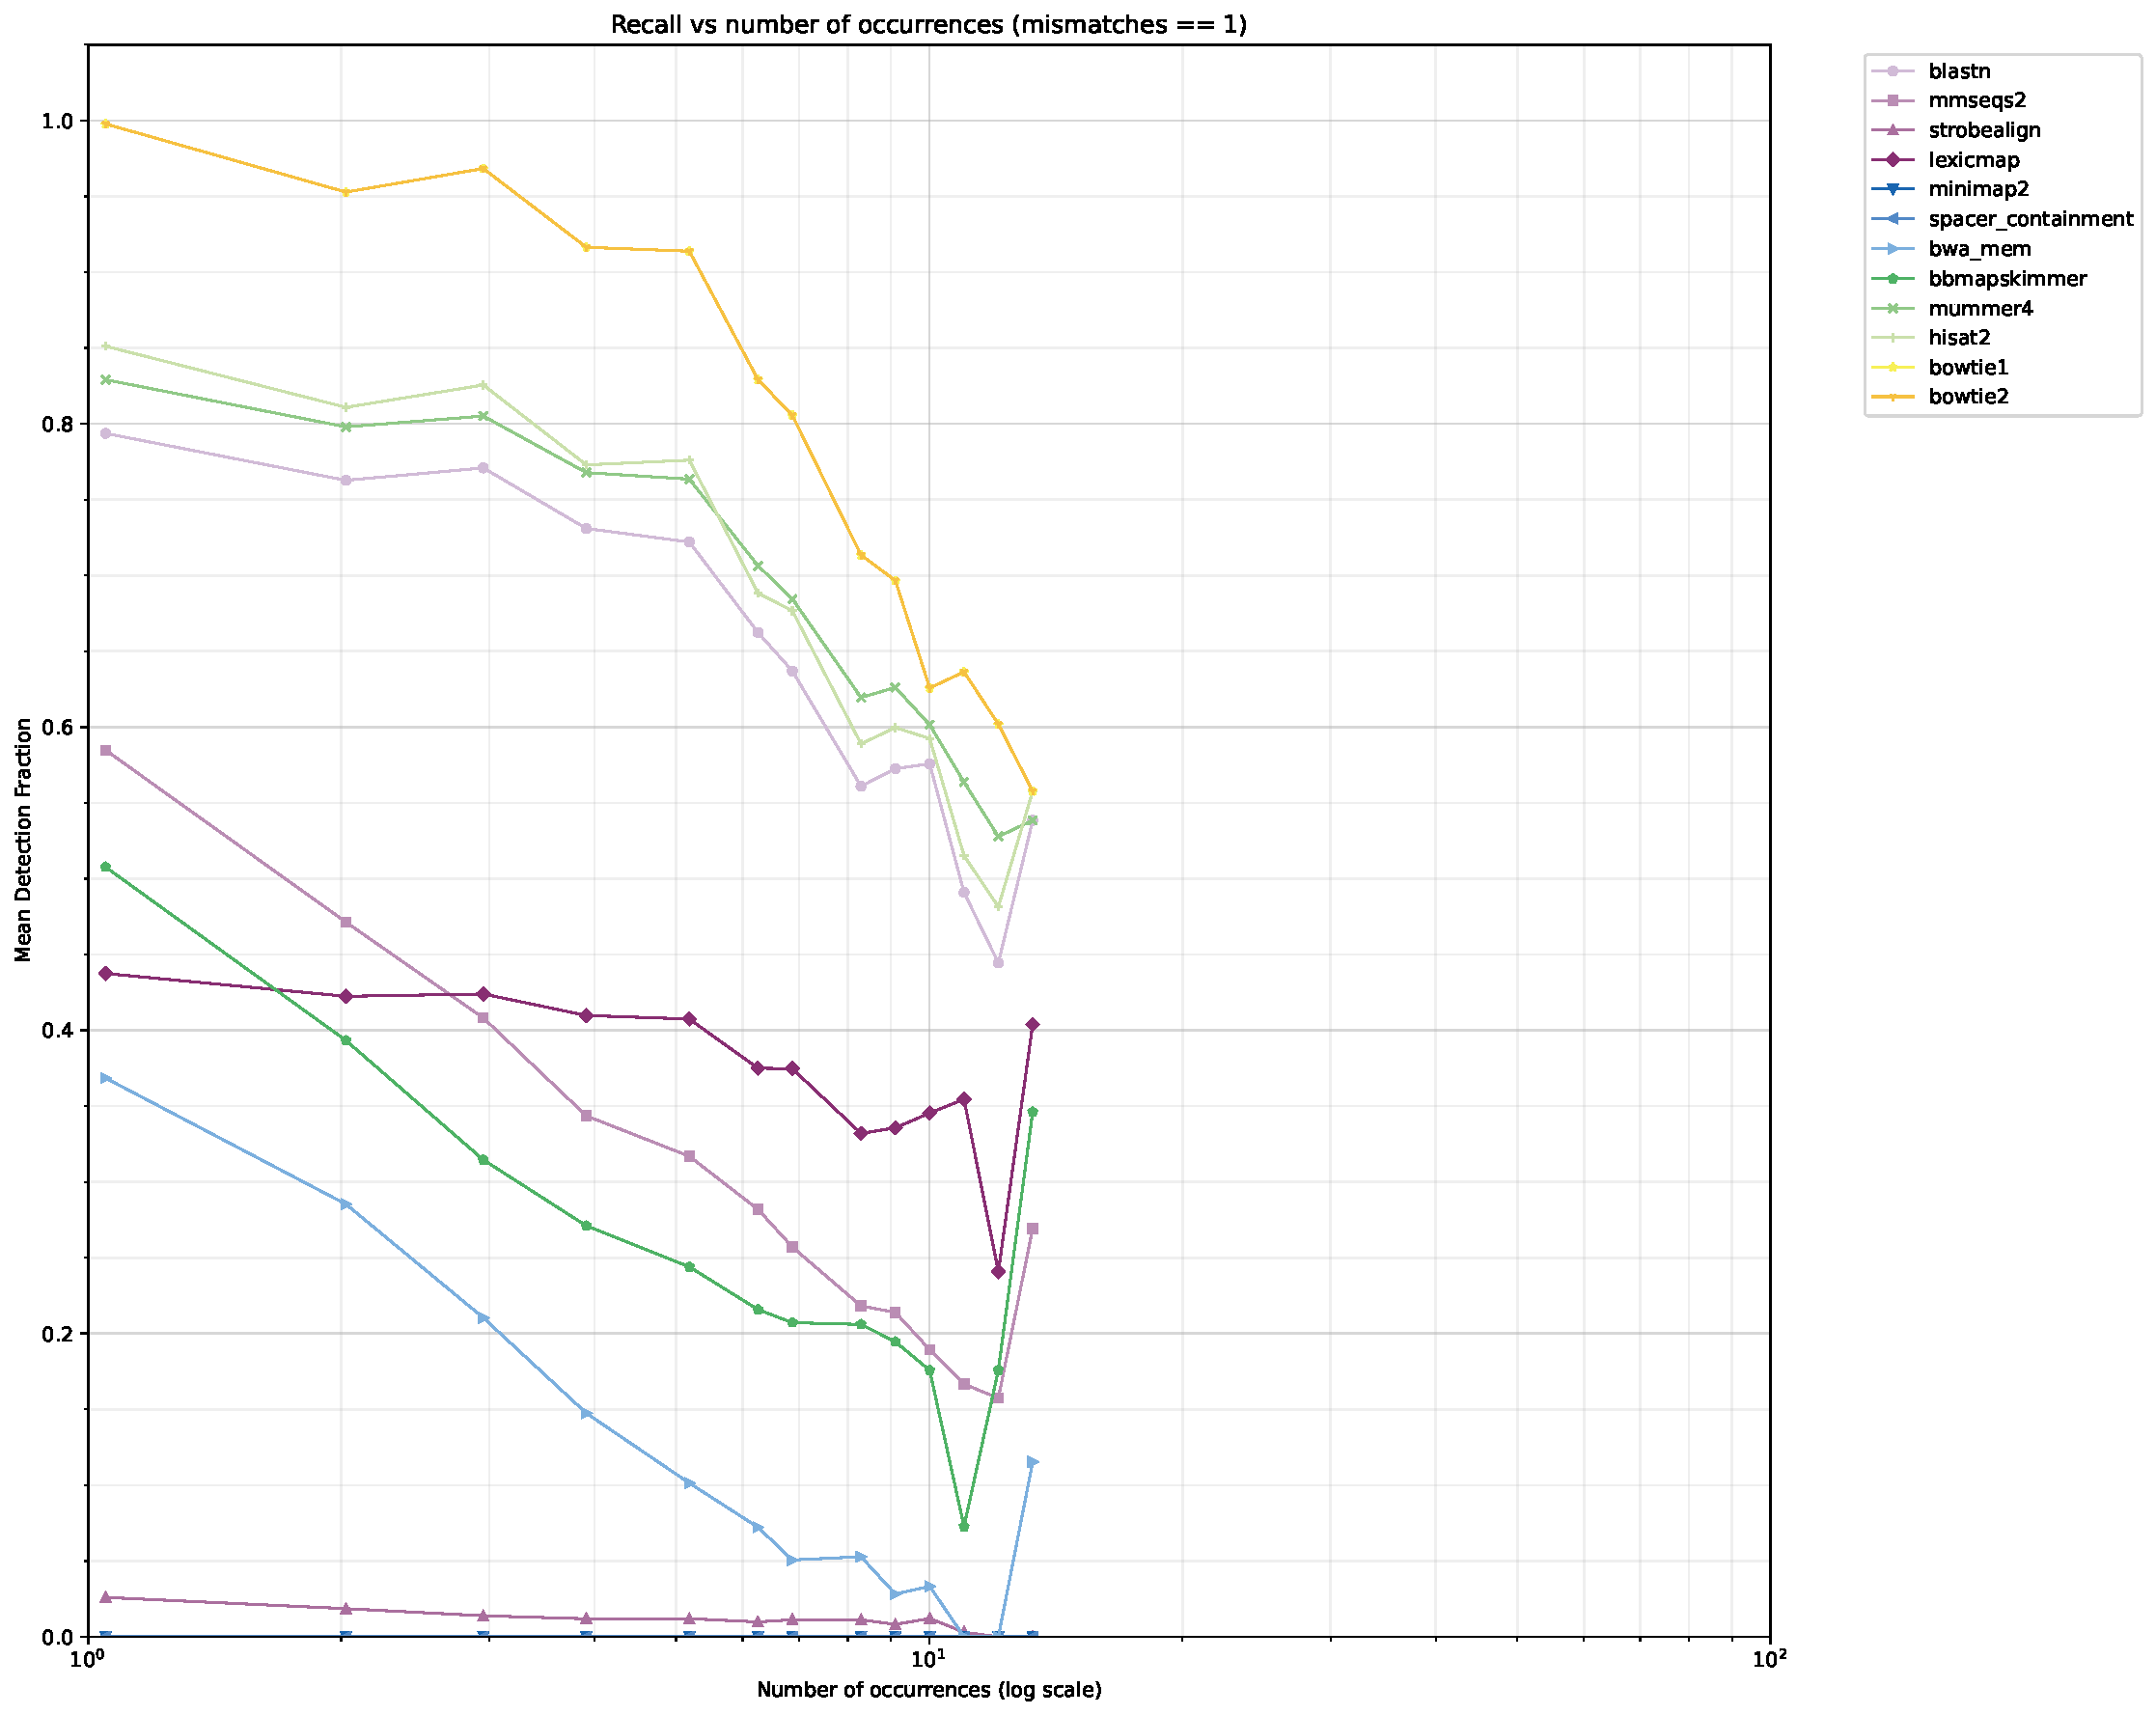
\includegraphics[keepaspectratio]{supplementary_files/mediabag/figures/supp/simulated_recall_vs_occurrences_with_contig_id_exact_nm_1.pdf}}

\begin{enumerate}
\def\labelenumi{\arabic{enumi}.}
\setcounter{enumi}{2}
\tightlist
\item
  exactly 2 mismatches
\end{enumerate}

\pandocbounded{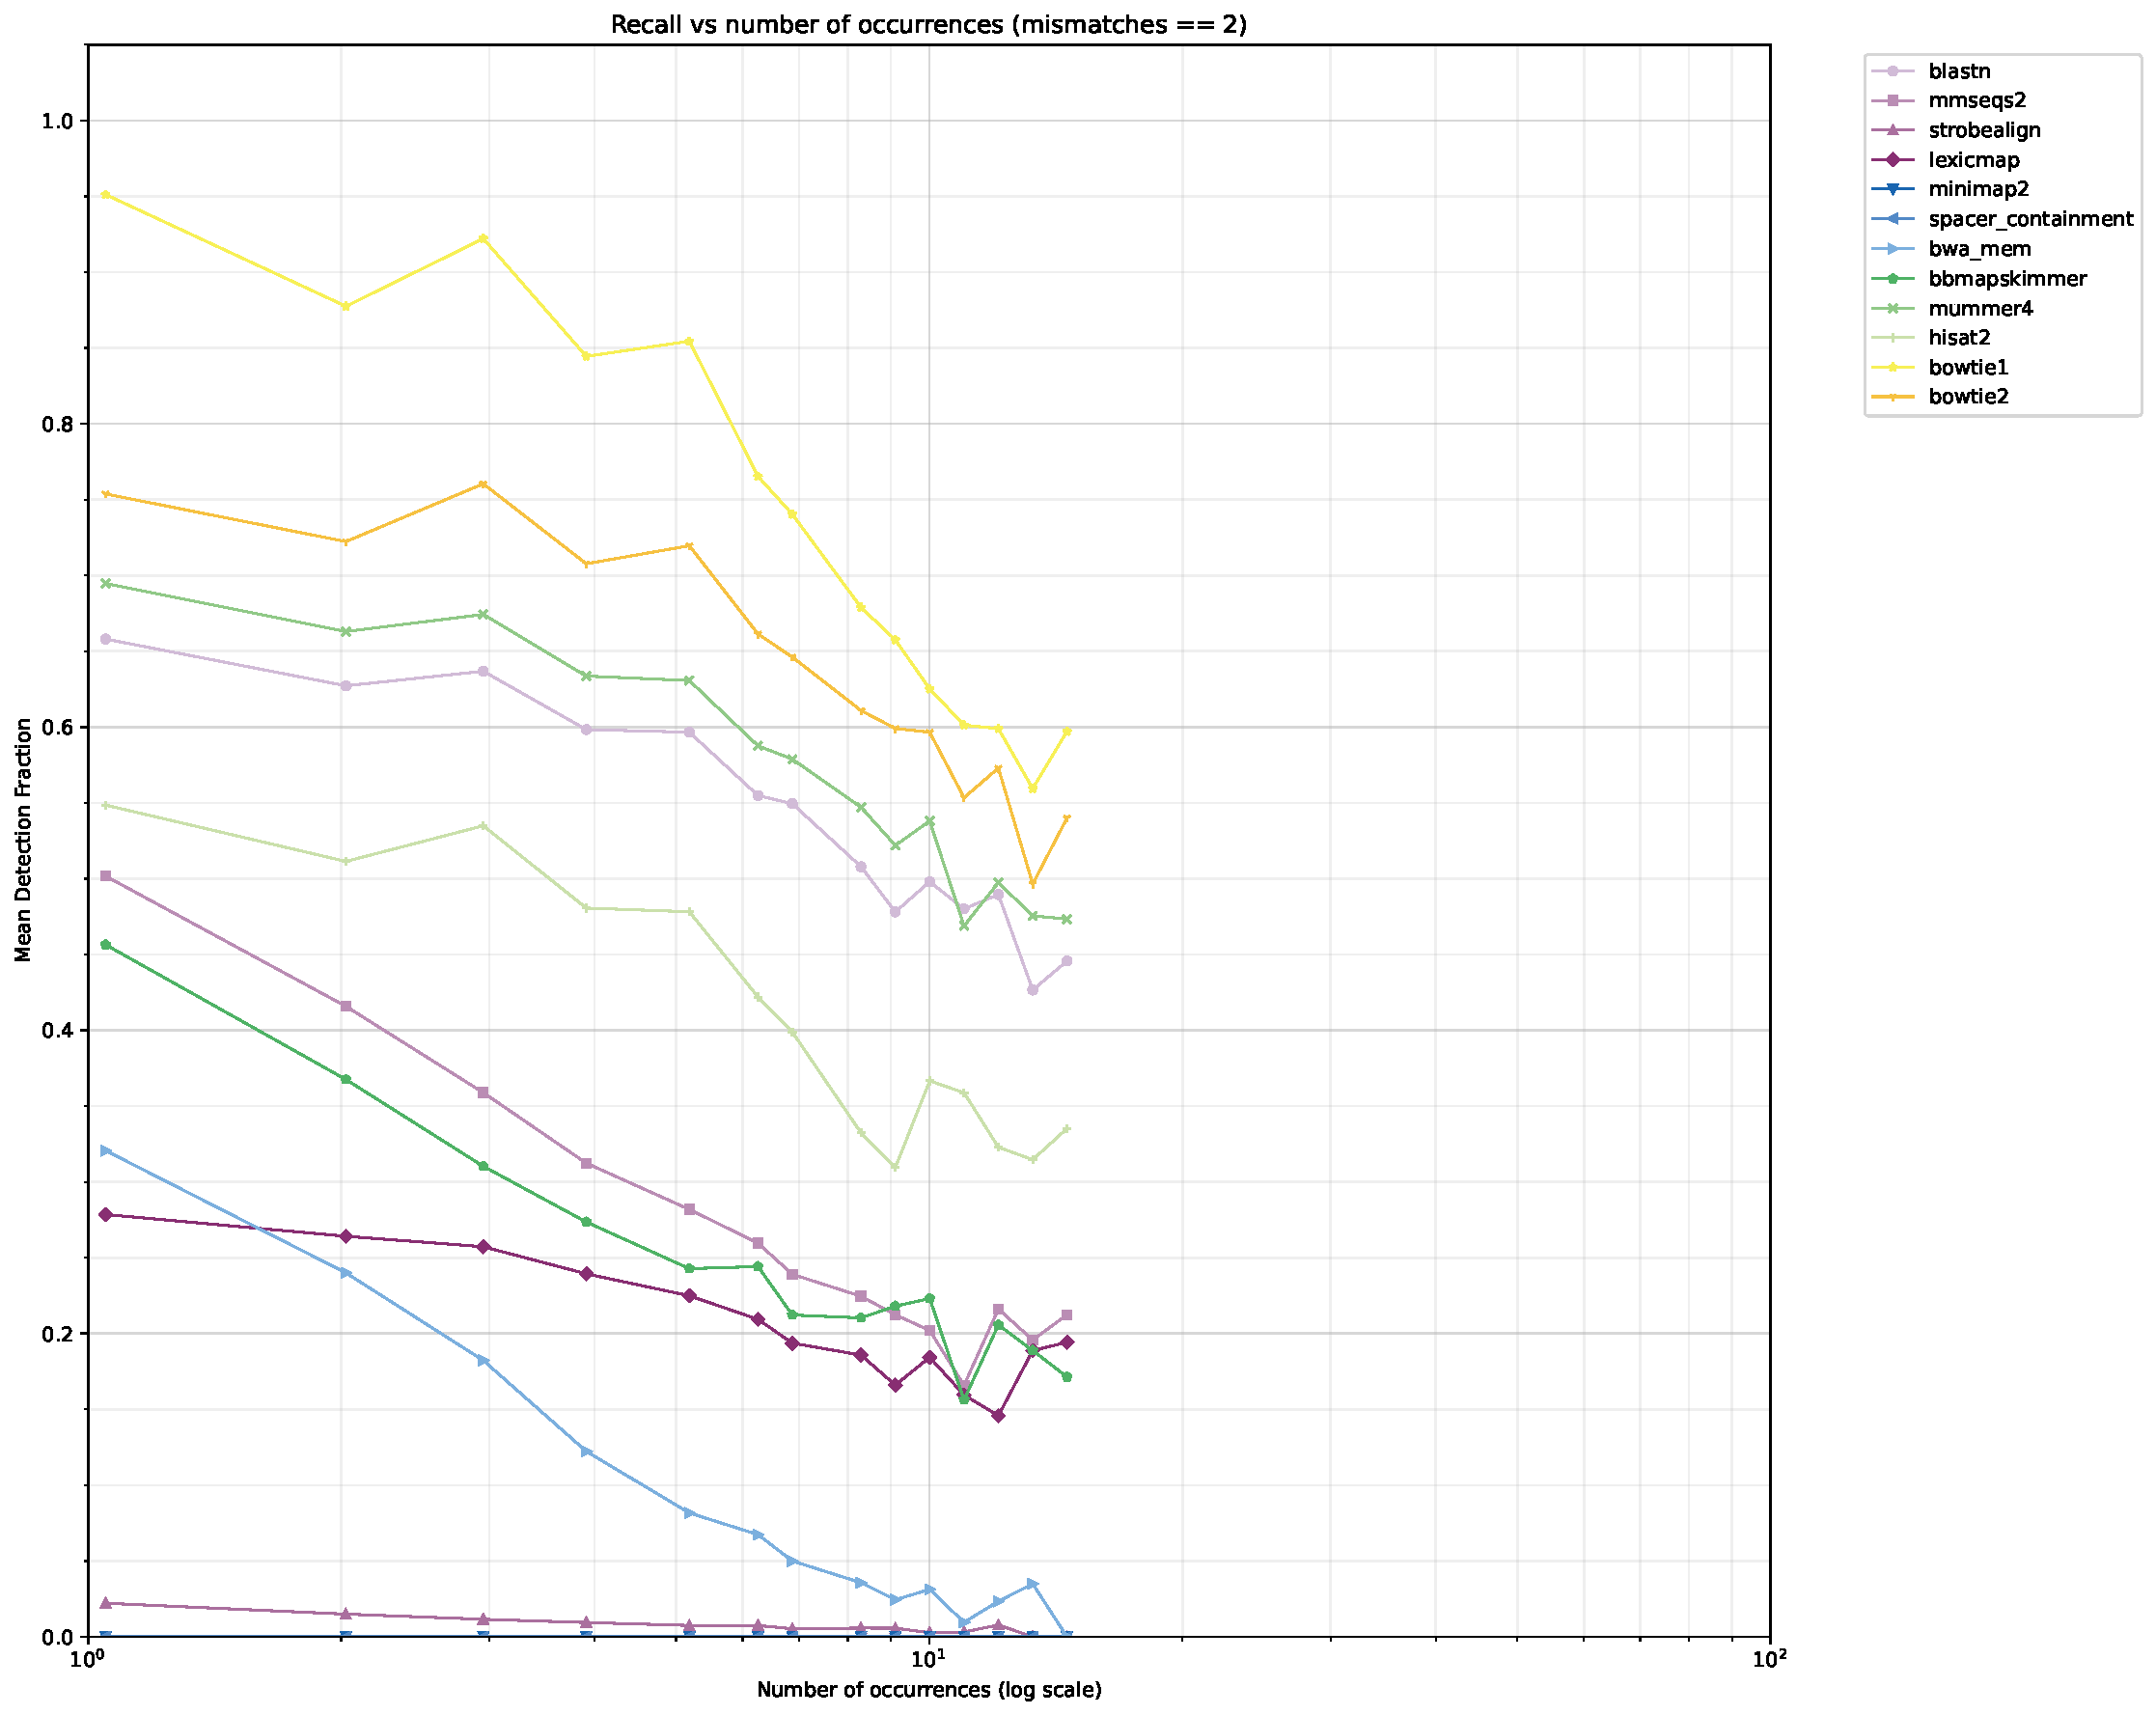
\includegraphics[keepaspectratio]{supplementary_files/mediabag/figures/supp/simulated_recall_vs_occurrences_with_contig_id_exact_nm_2.pdf}}

\begin{enumerate}
\def\labelenumi{\arabic{enumi}.}
\setcounter{enumi}{3}
\tightlist
\item
  exactly 3 mismatches
\end{enumerate}

\pandocbounded{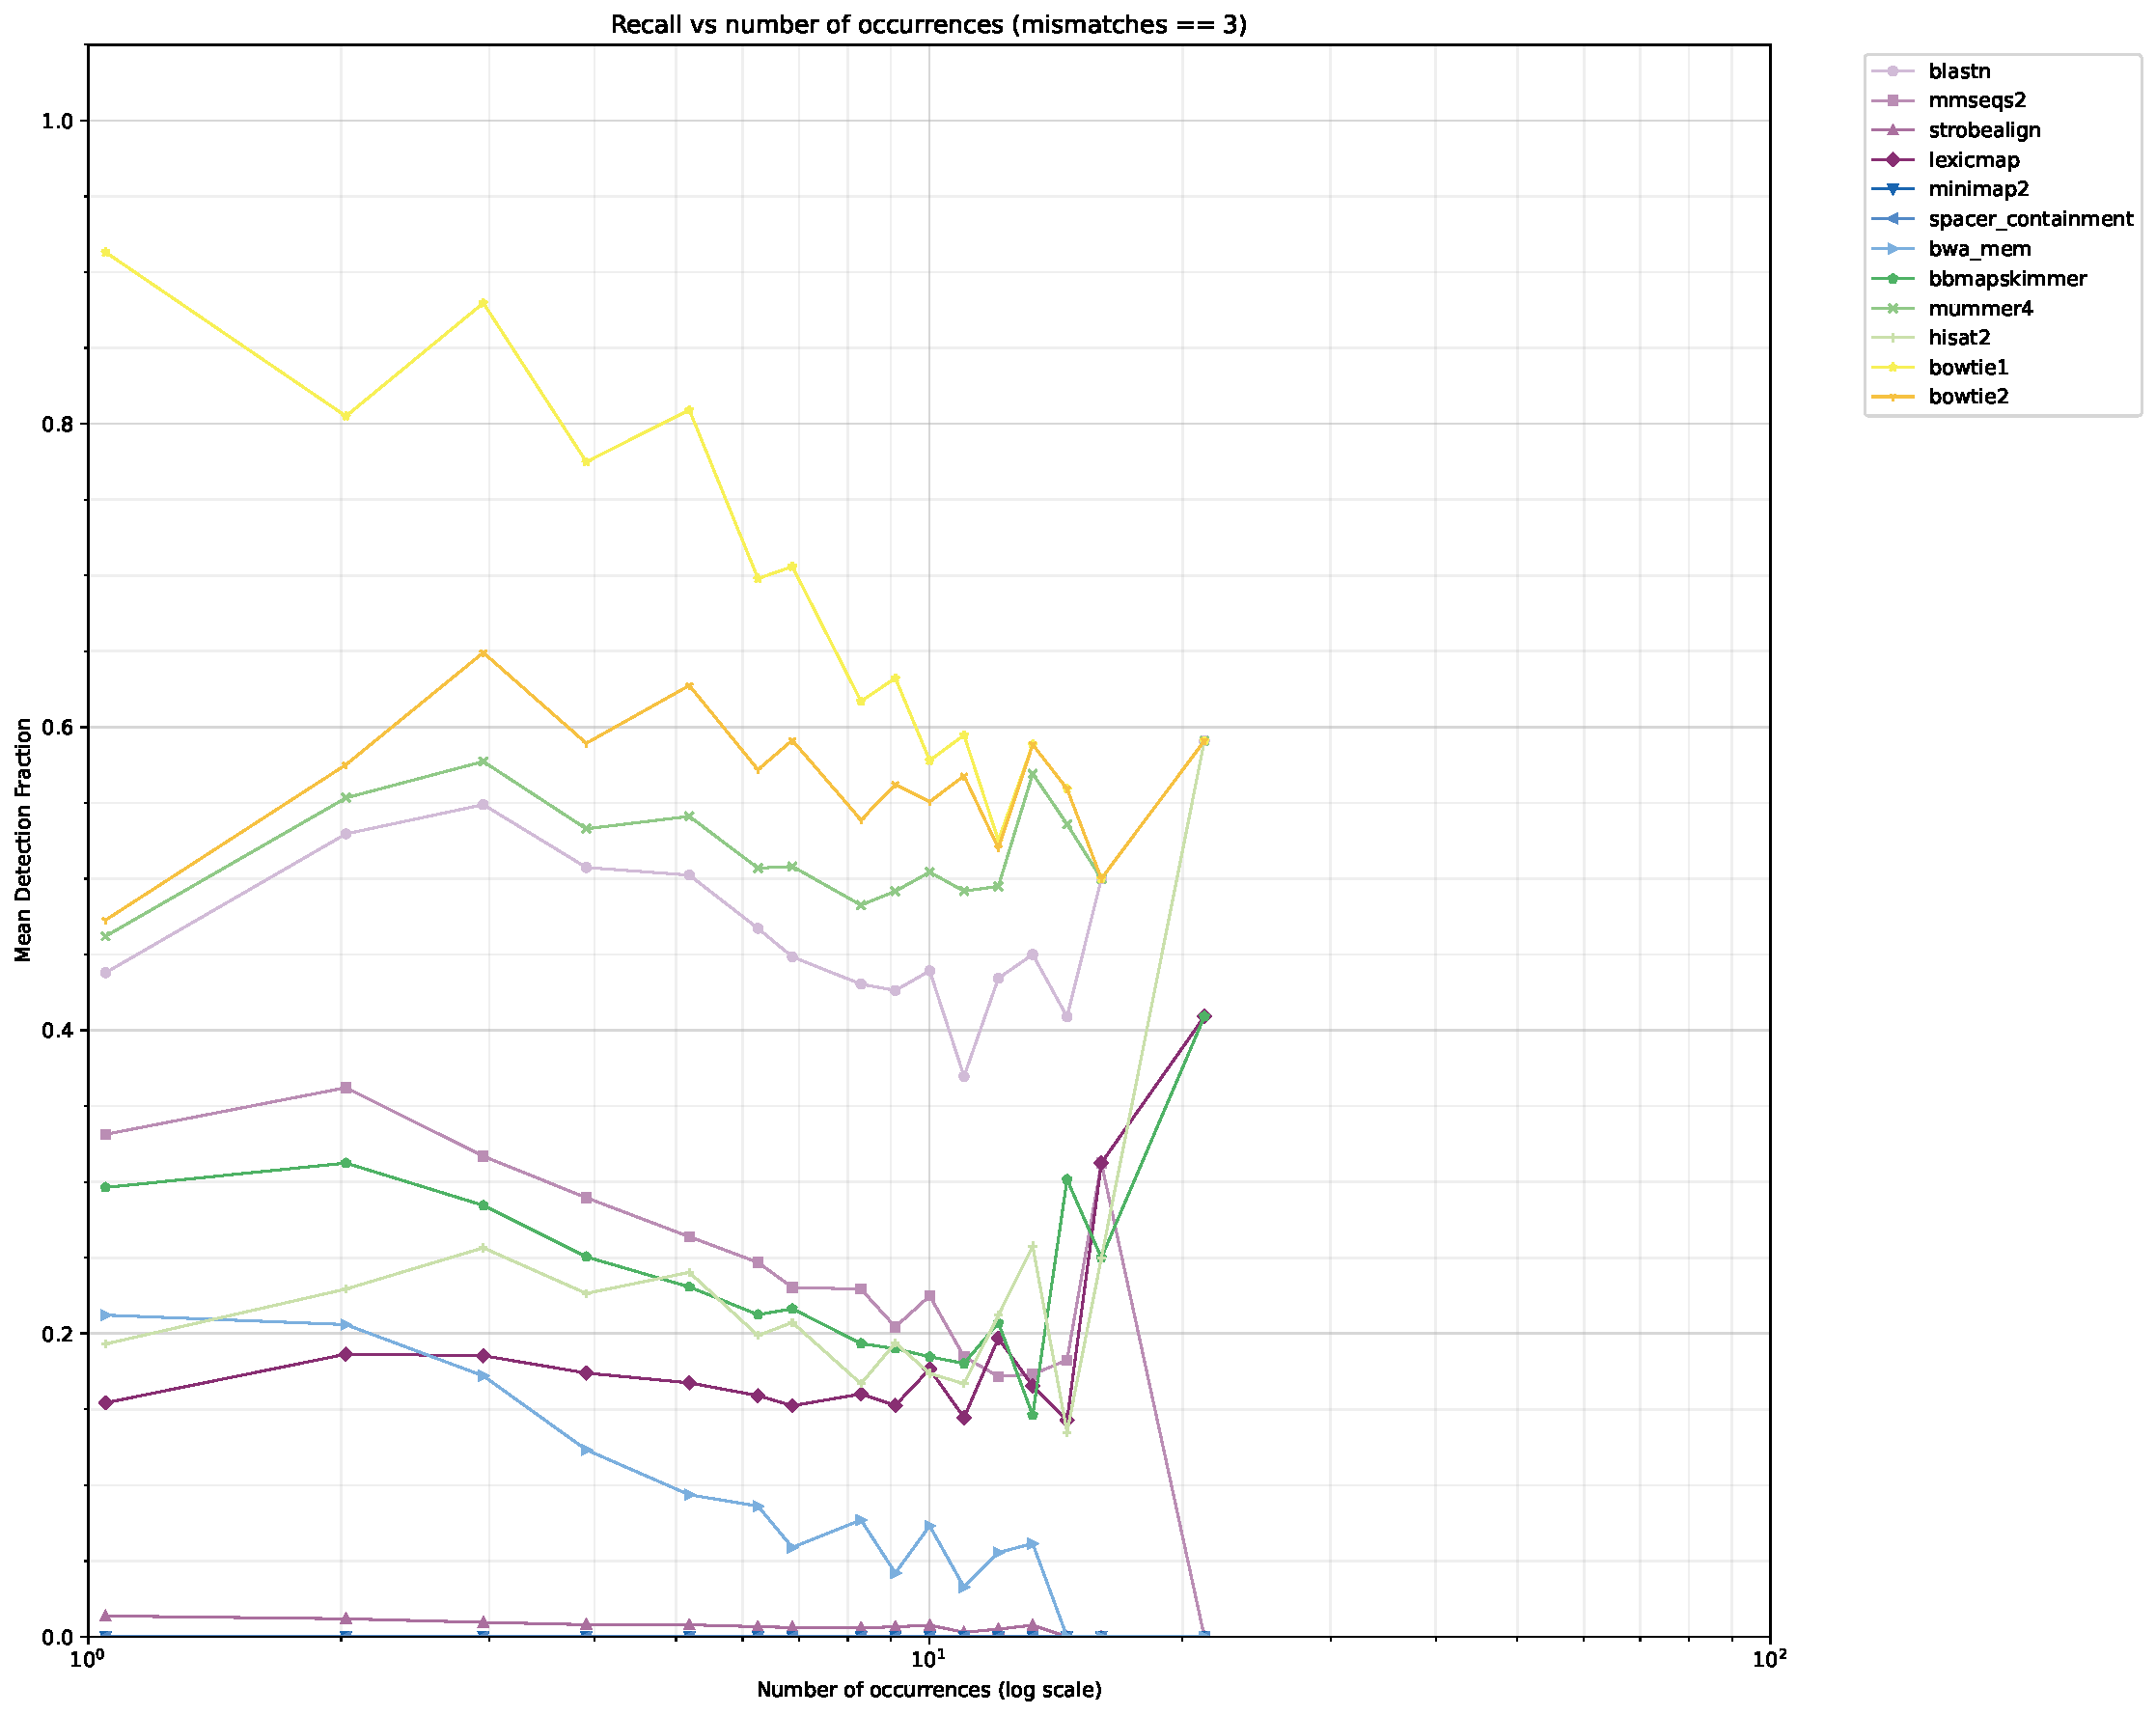
\includegraphics[keepaspectratio]{supplementary_files/mediabag/figures/supp/simulated_recall_vs_occurrences_with_contig_id_exact_nm_3.pdf}}

\paragraph{B. up to 1 and 3 mismatches, in a contig independent
manner}\label{b.-up-to-1-and-3-mismatches-in-a-contig-independent-manner}

Per contig independent manner means that the recall measure is the
fraction of occurences each tool identified out of the total number of
times the spacer occurs in the reference file (regardless of in which
contig).\\
1. up to 1 mismatches

\pandocbounded{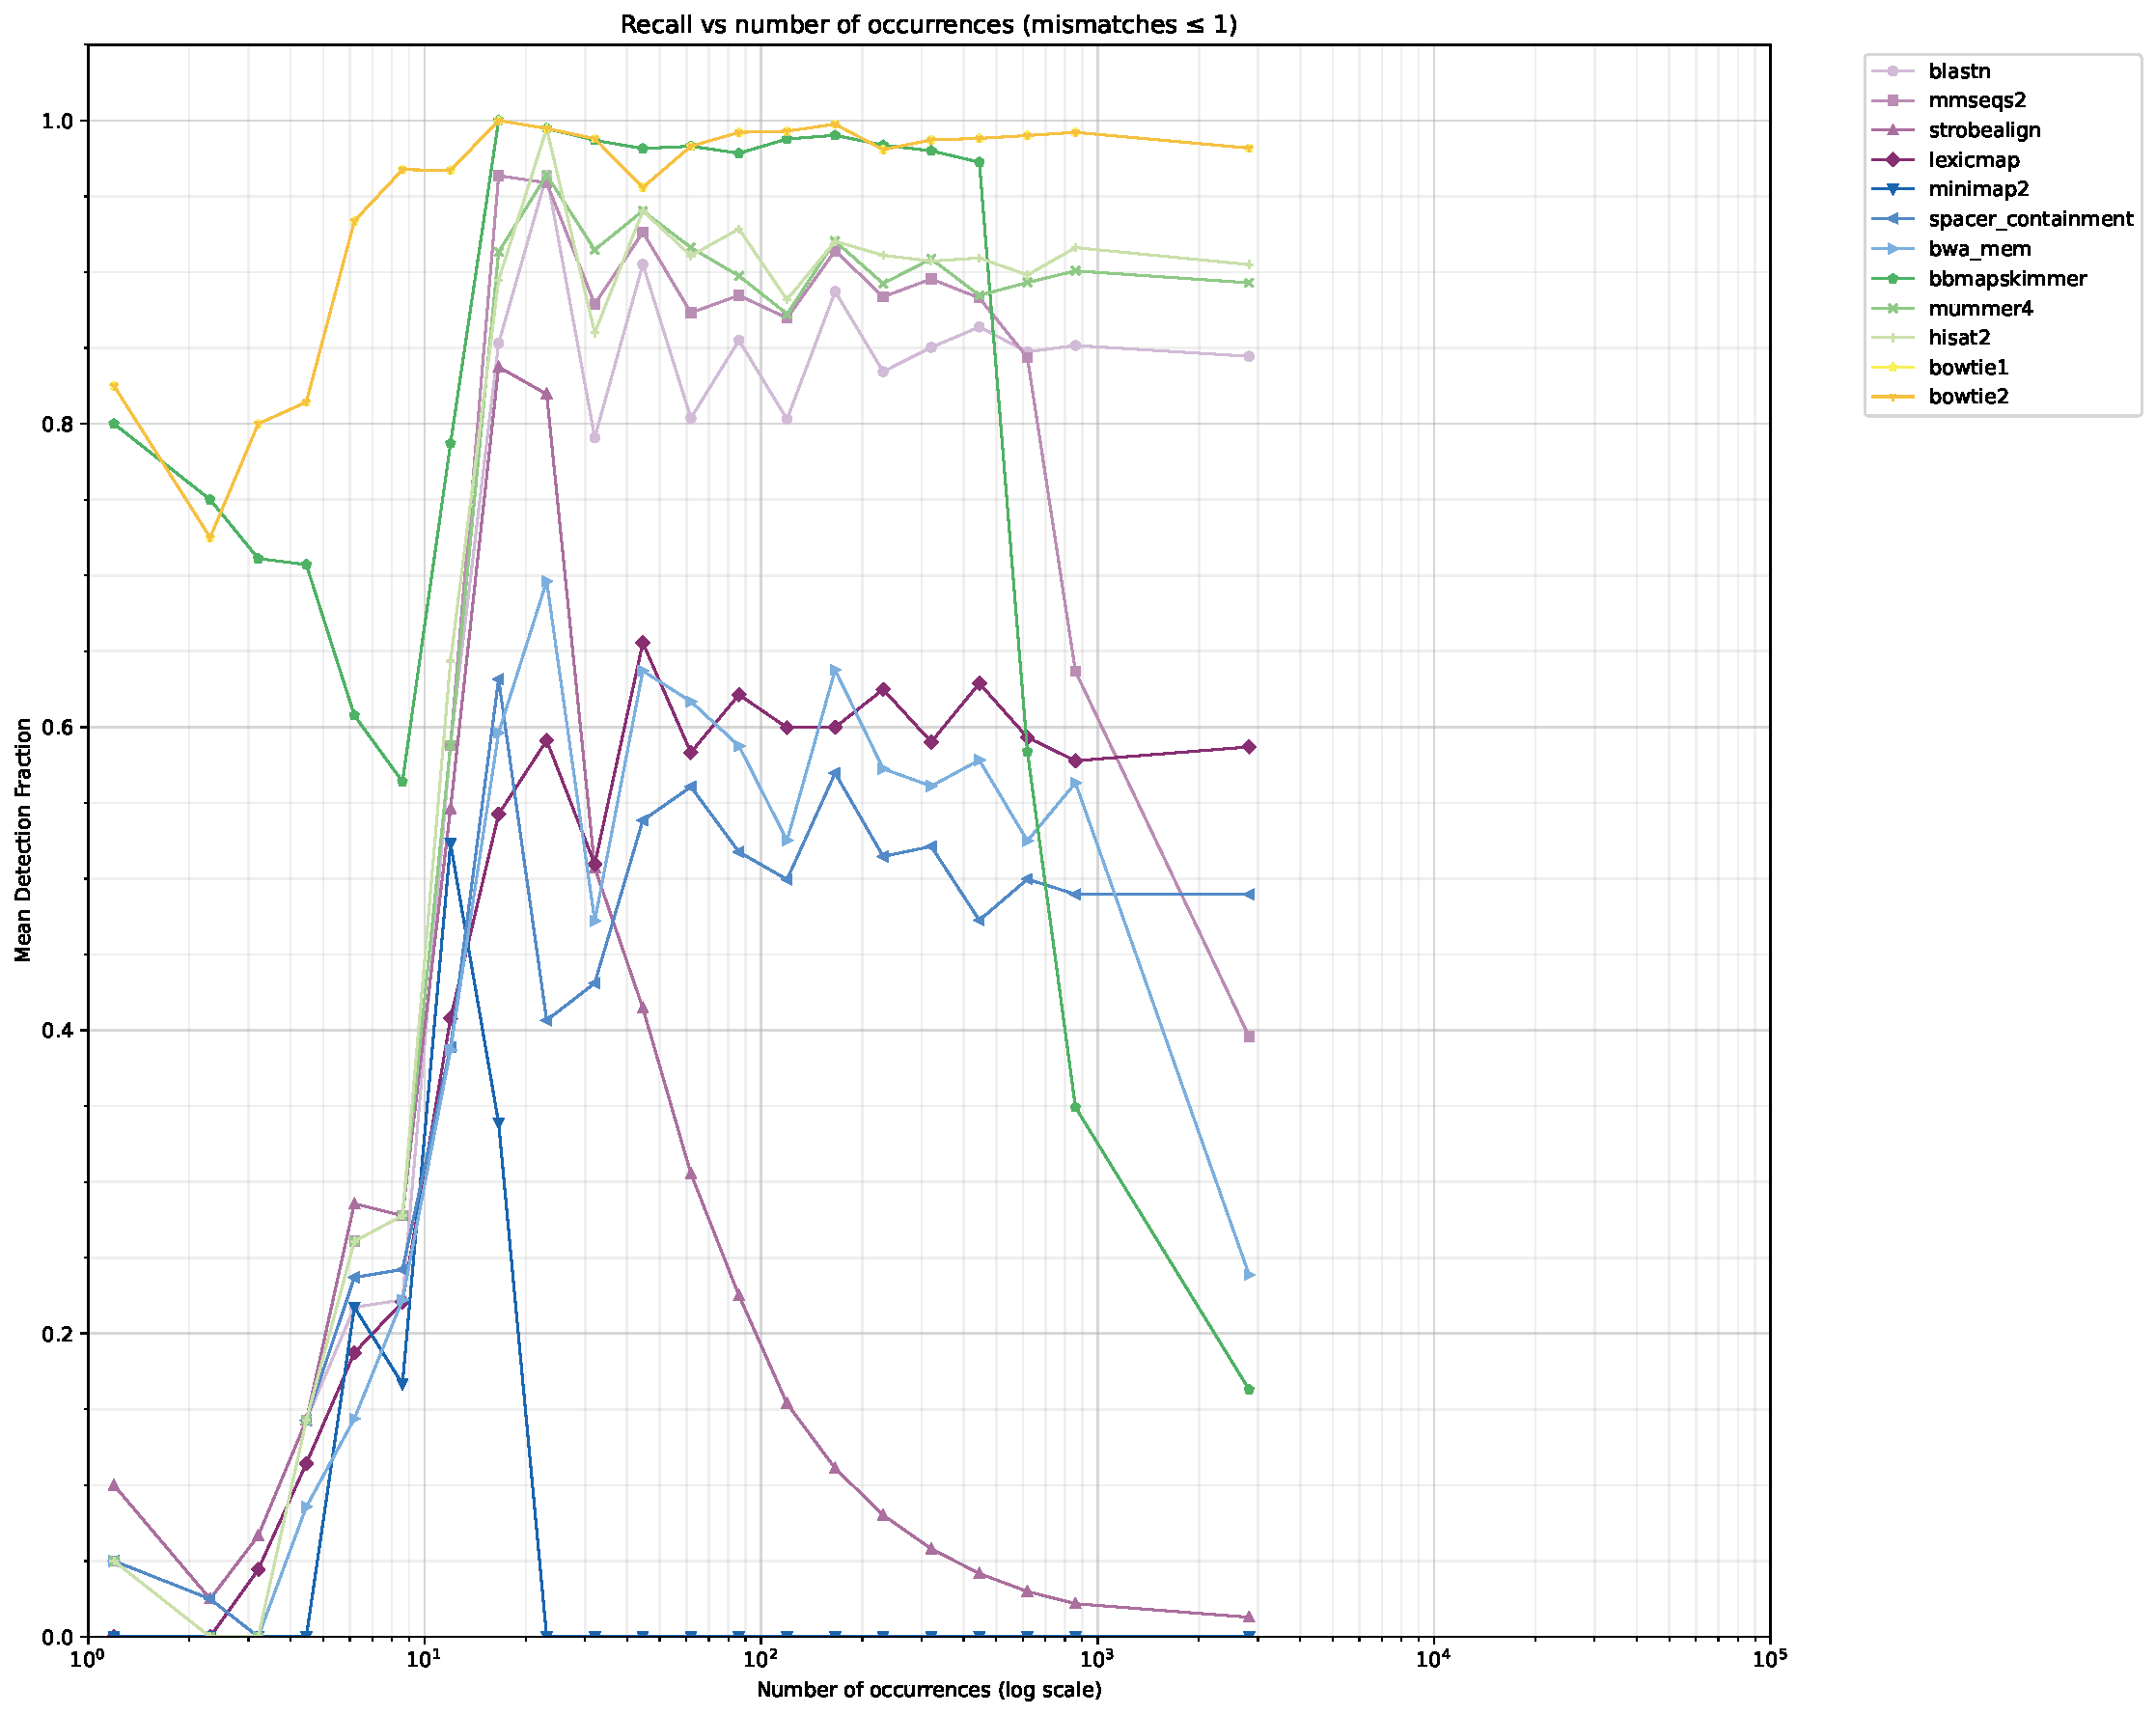
\includegraphics[keepaspectratio]{supplementary_files/mediabag/figures/supp/simulated_recall_vs_occurrences_max_nm_1.pdf}}

\begin{enumerate}
\def\labelenumi{\arabic{enumi}.}
\setcounter{enumi}{1}
\tightlist
\item
  up to 3 mismatches
\end{enumerate}

\pandocbounded{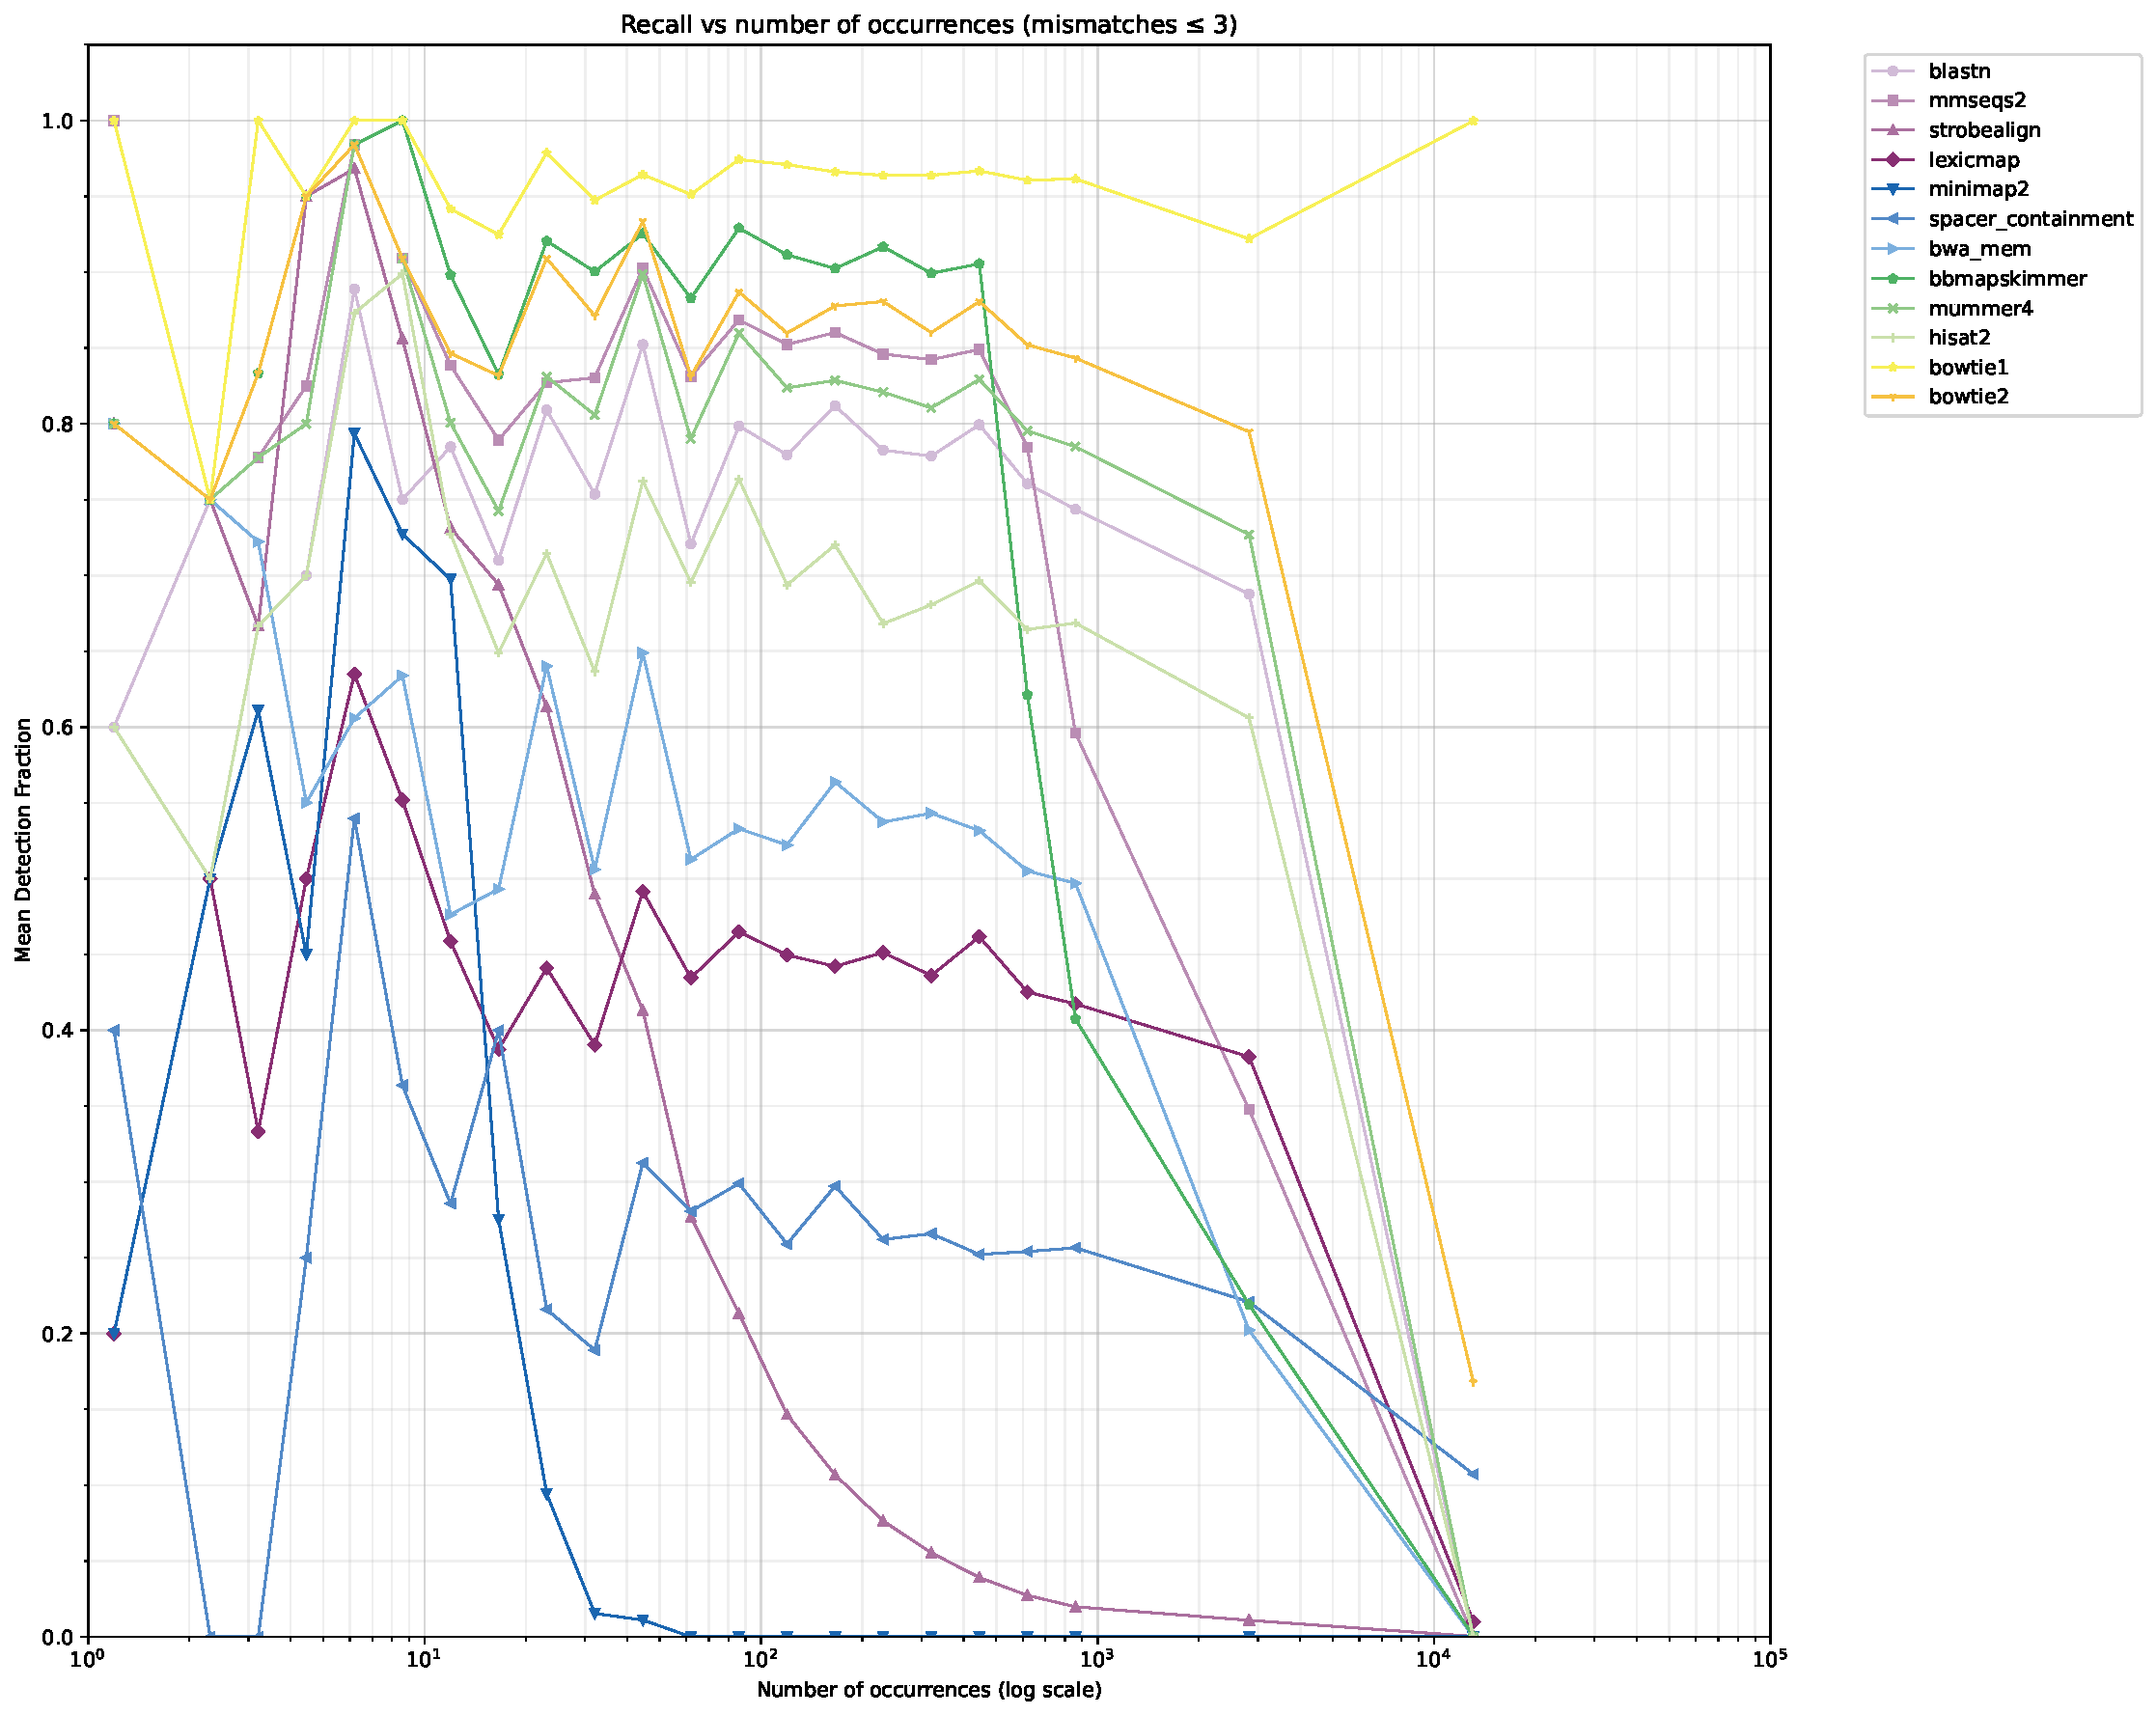
\includegraphics[keepaspectratio]{supplementary_files/mediabag/figures/supp/simulated_recall_vs_occurrences_max_nm_3.pdf}}

\subsubsection{Supplementary figure 5.}\label{supplementary-figure-5.}

Tool recall versus occurrence frequency for \textbf{IMG/VR4 dataset}.\\
Similar to main text figure, except for exact values for different
mismatch thresholds (0-3). \#\#\#\# A. 0 mismatches

\pandocbounded{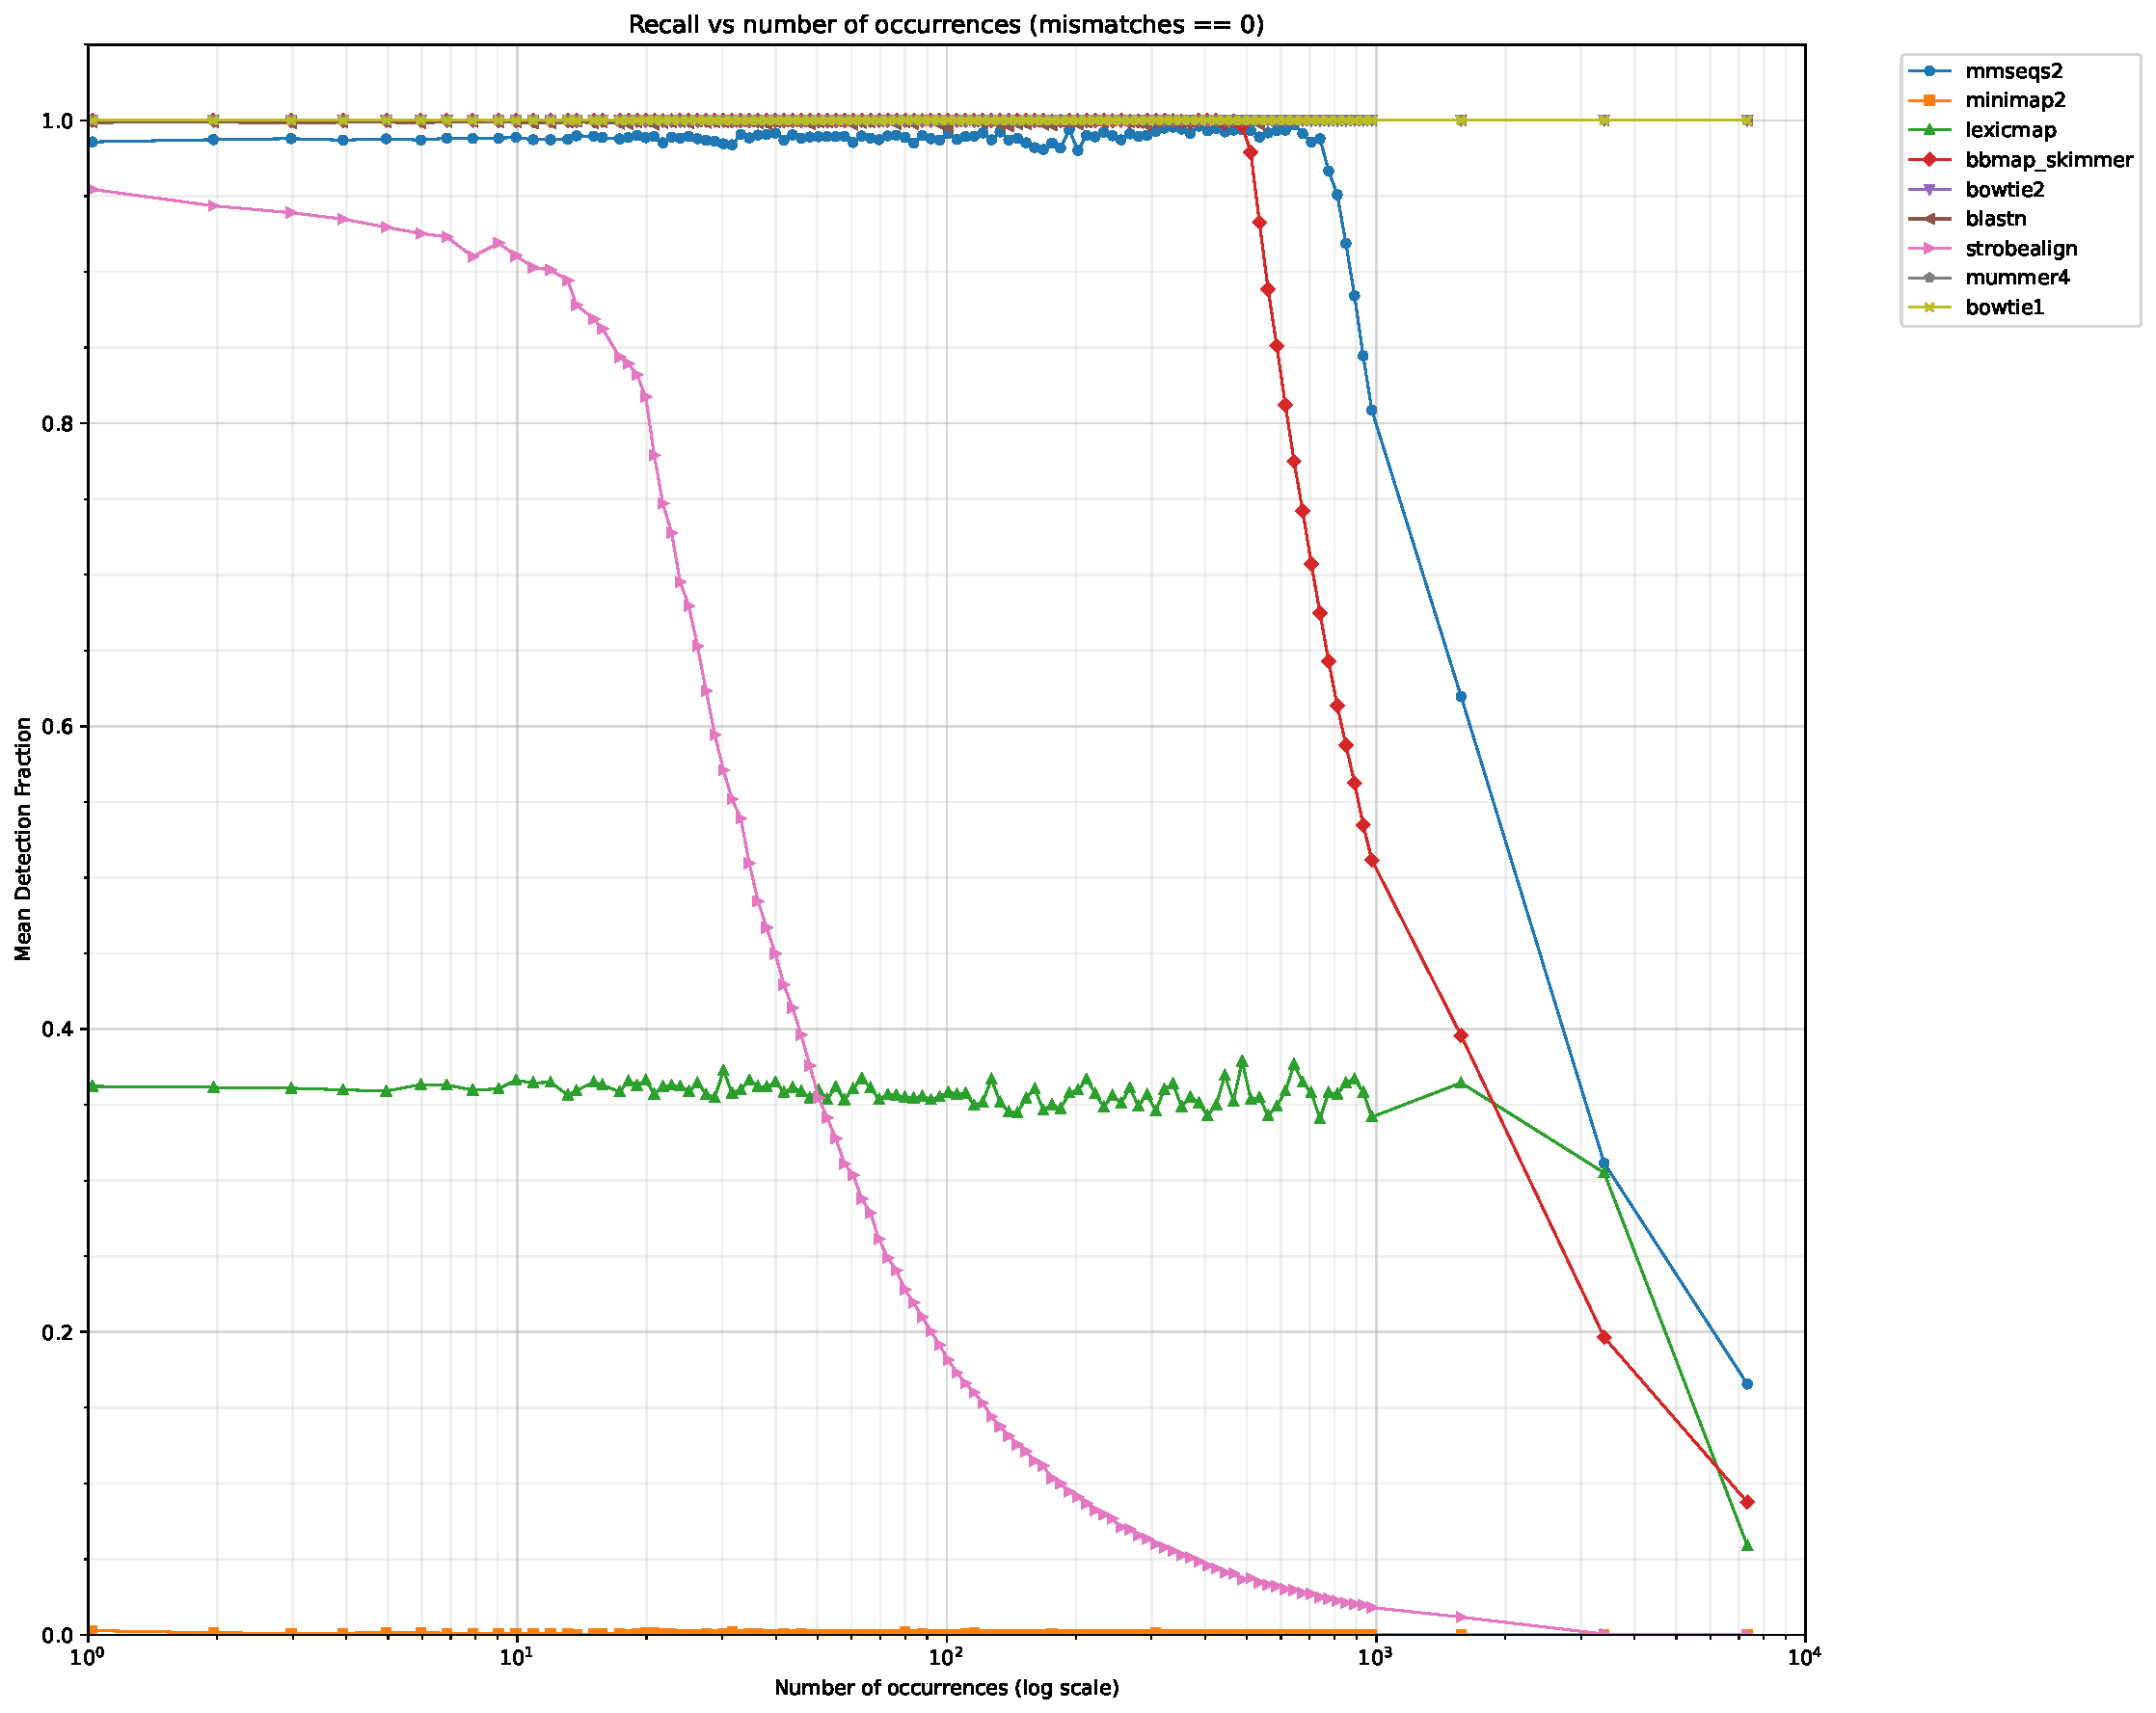
\includegraphics[keepaspectratio]{supplementary_files/mediabag/figures/supp/real_data_recall_vs_occurrences_exact_nm_0.pdf}}

\paragraph{B. 1 mismatch}\label{b.-1-mismatch}

\pandocbounded{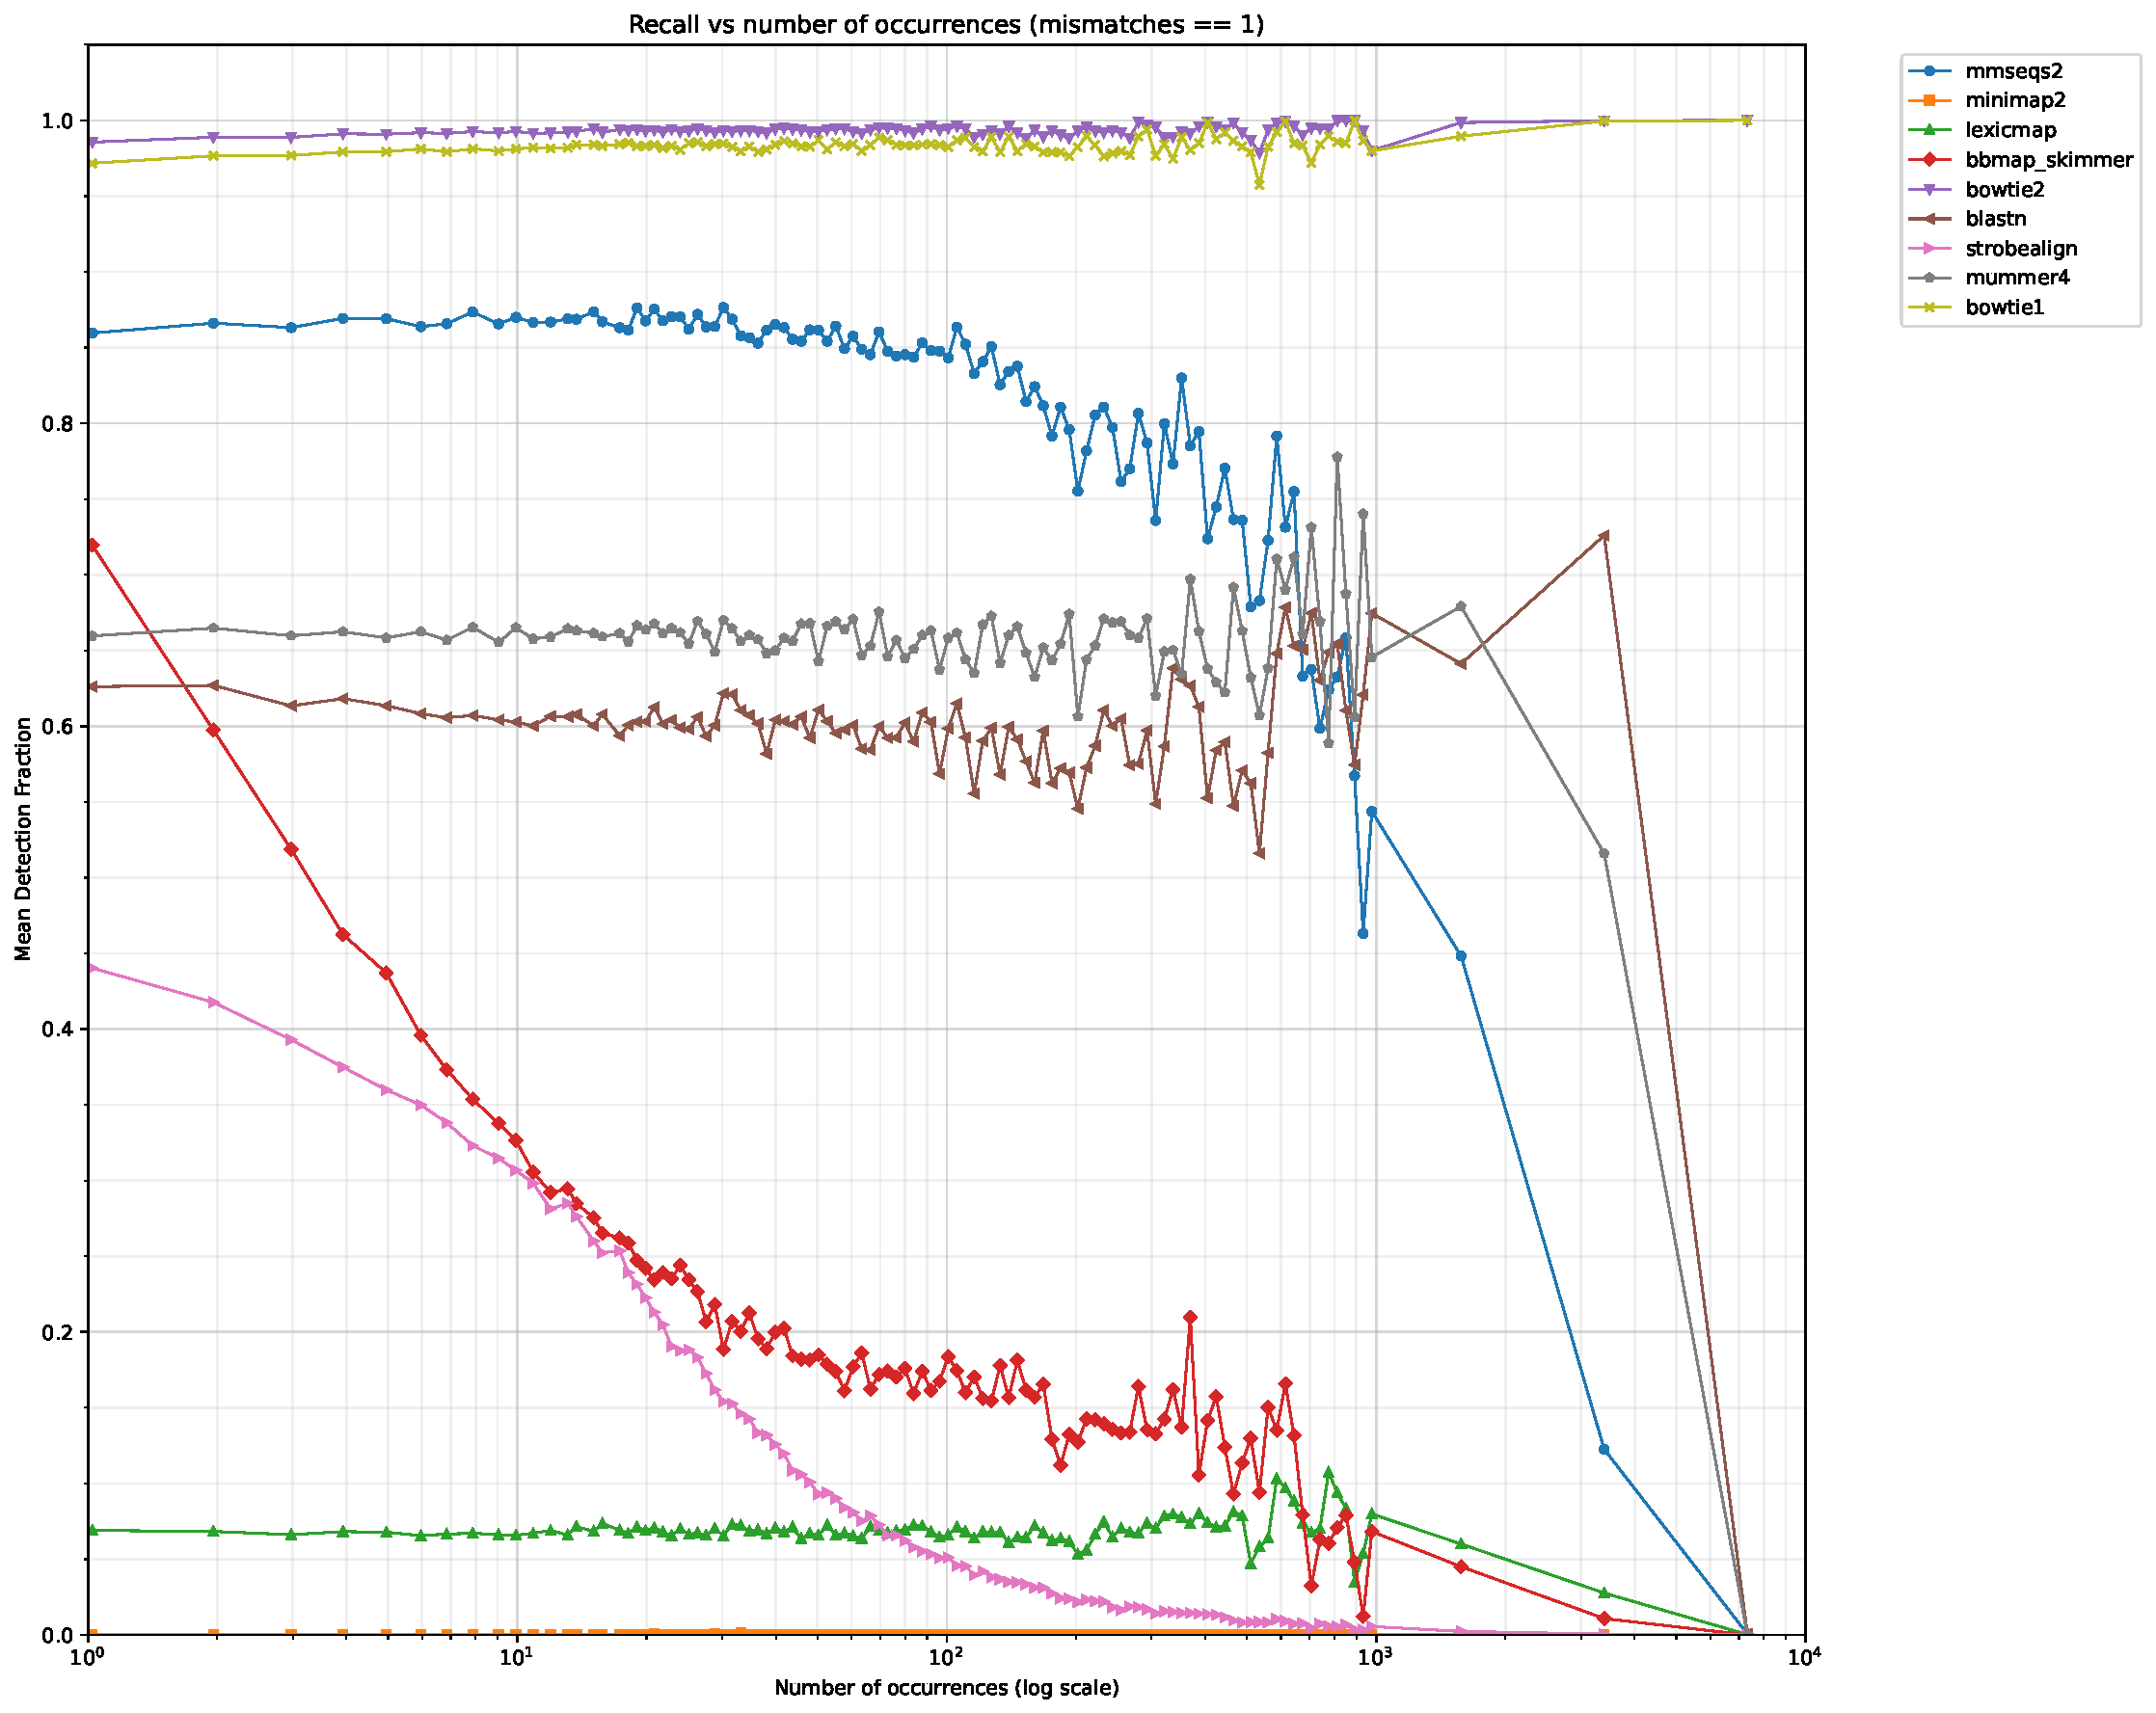
\includegraphics[keepaspectratio]{supplementary_files/mediabag/figures/supp/real_data_recall_vs_occurrences_exact_nm_1.pdf}}

\paragraph{C. 2 mismatches}\label{c.-2-mismatches}

\pandocbounded{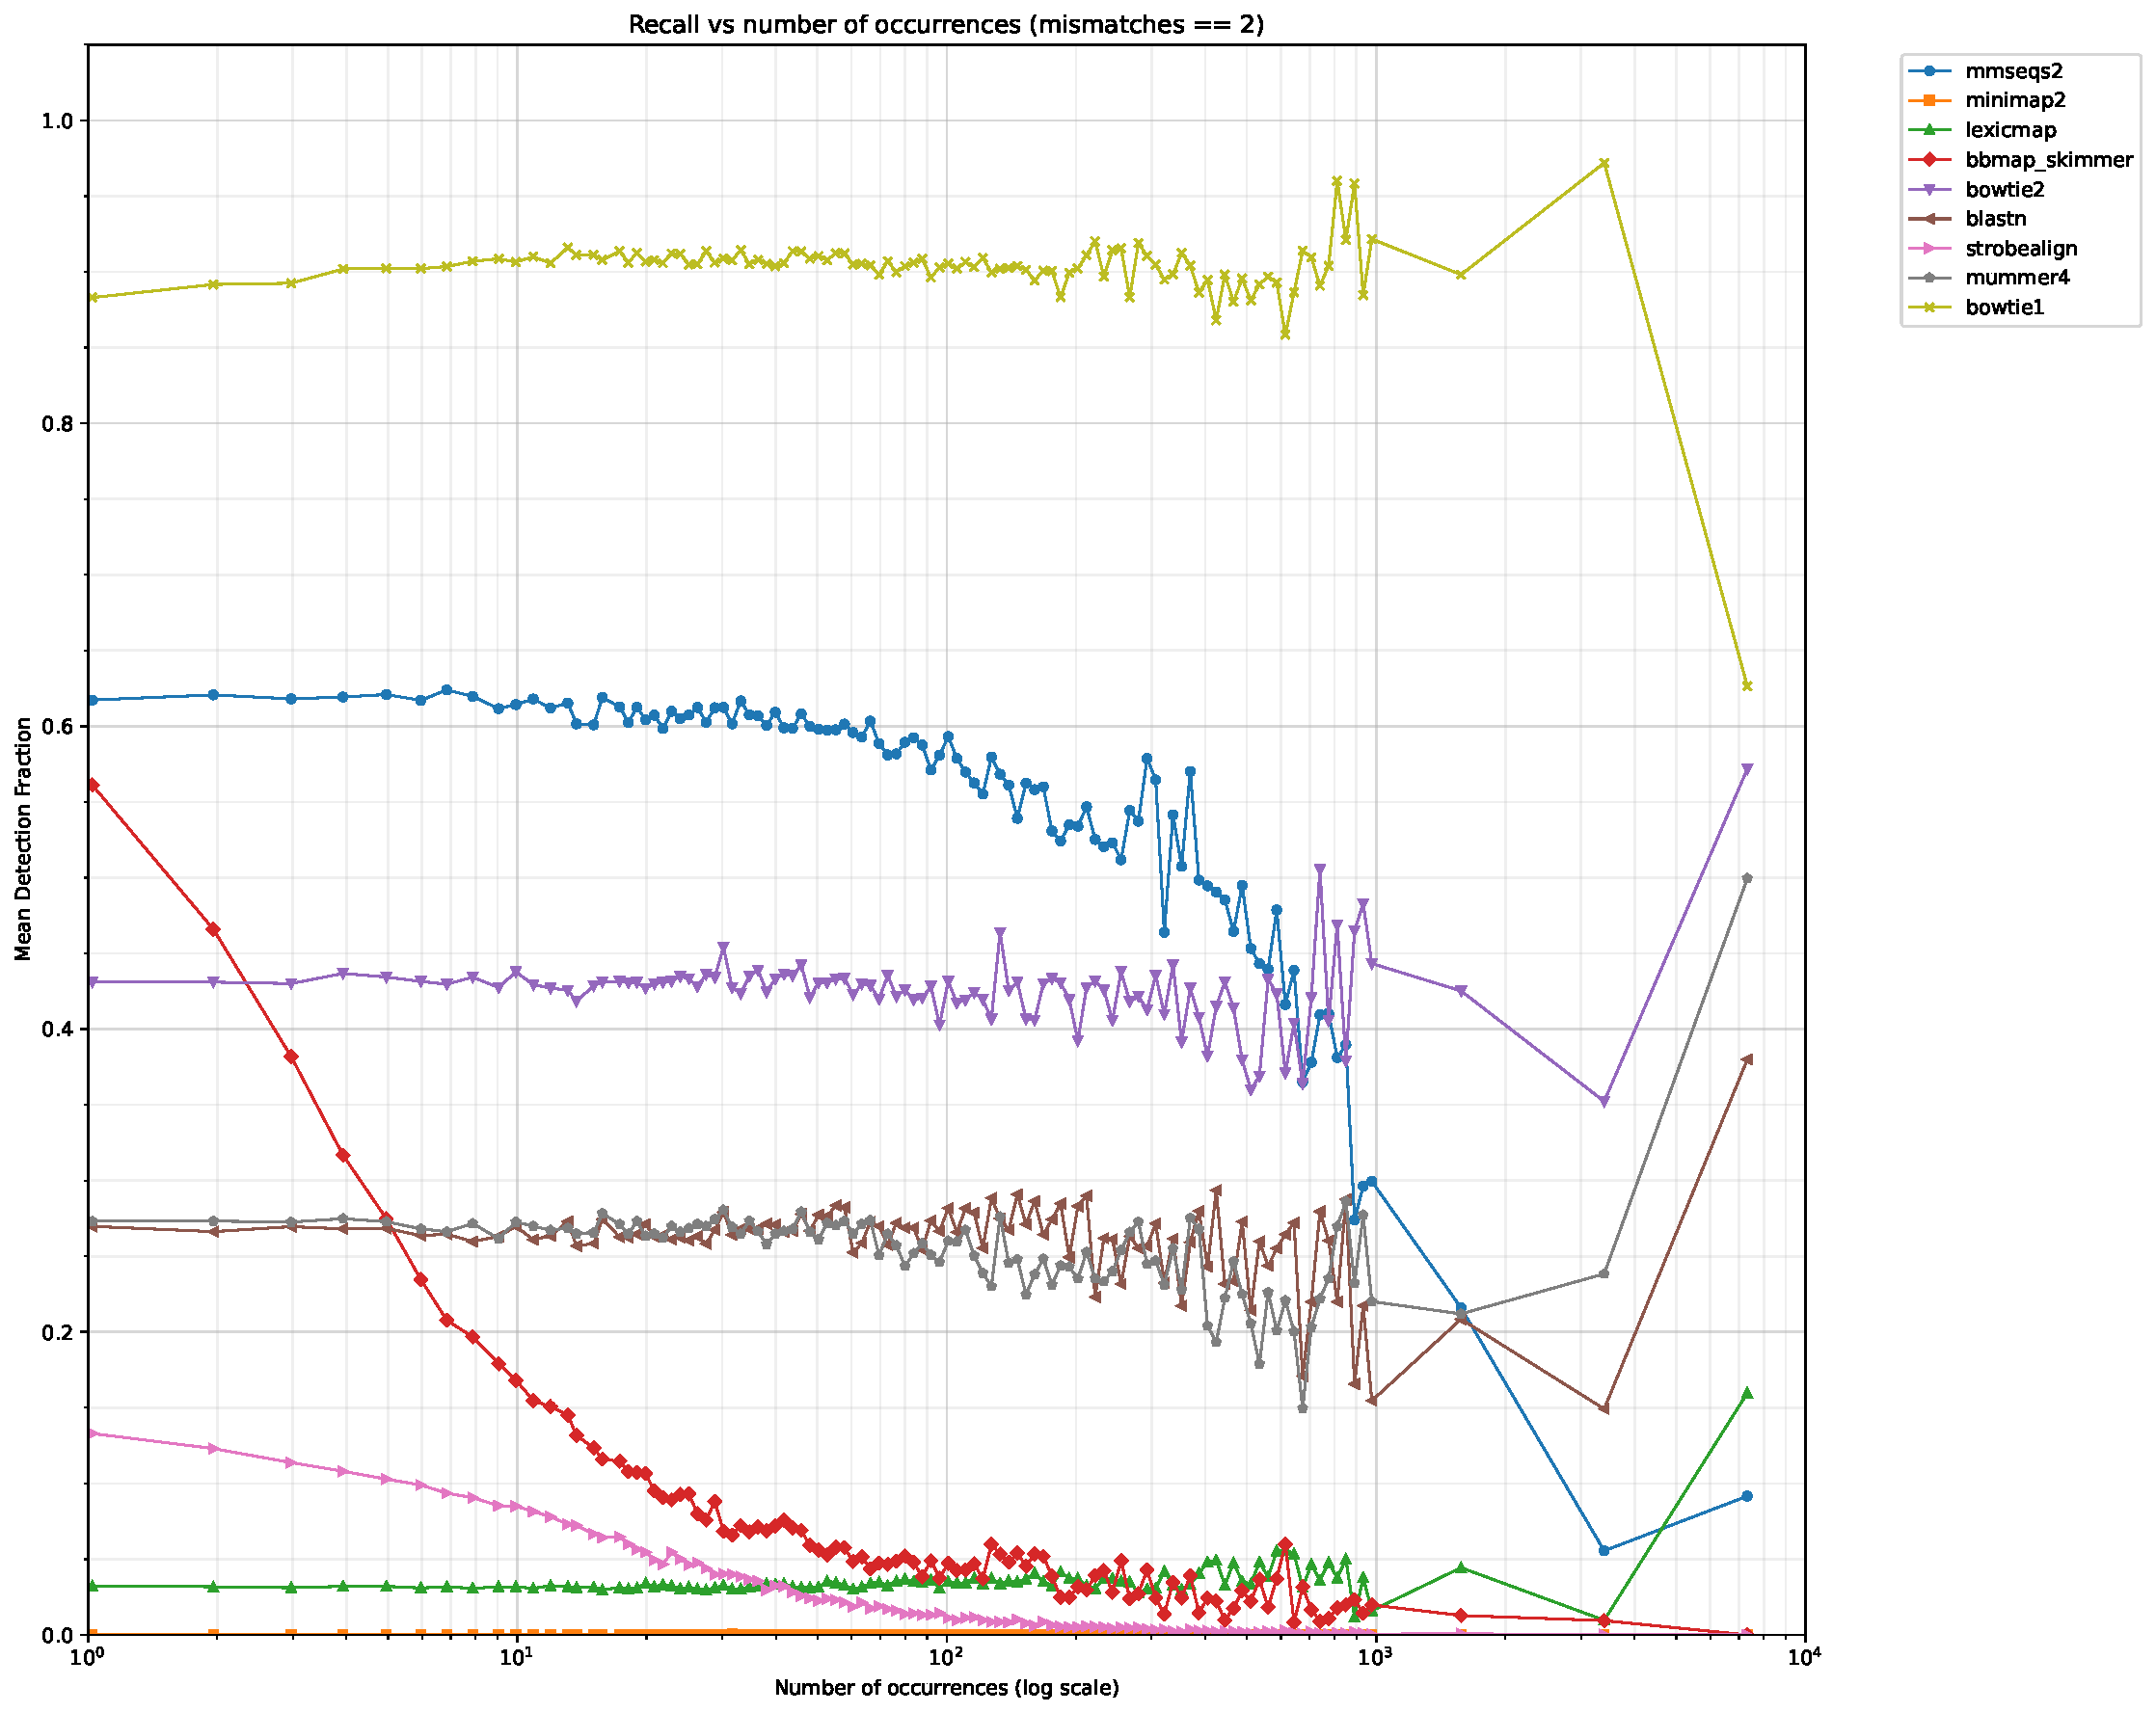
\includegraphics[keepaspectratio]{supplementary_files/mediabag/figures/supp/real_data_recall_vs_occurrences_exact_nm_2.pdf}}

\paragraph{D. 3 mismatches}\label{d.-3-mismatches}

\pandocbounded{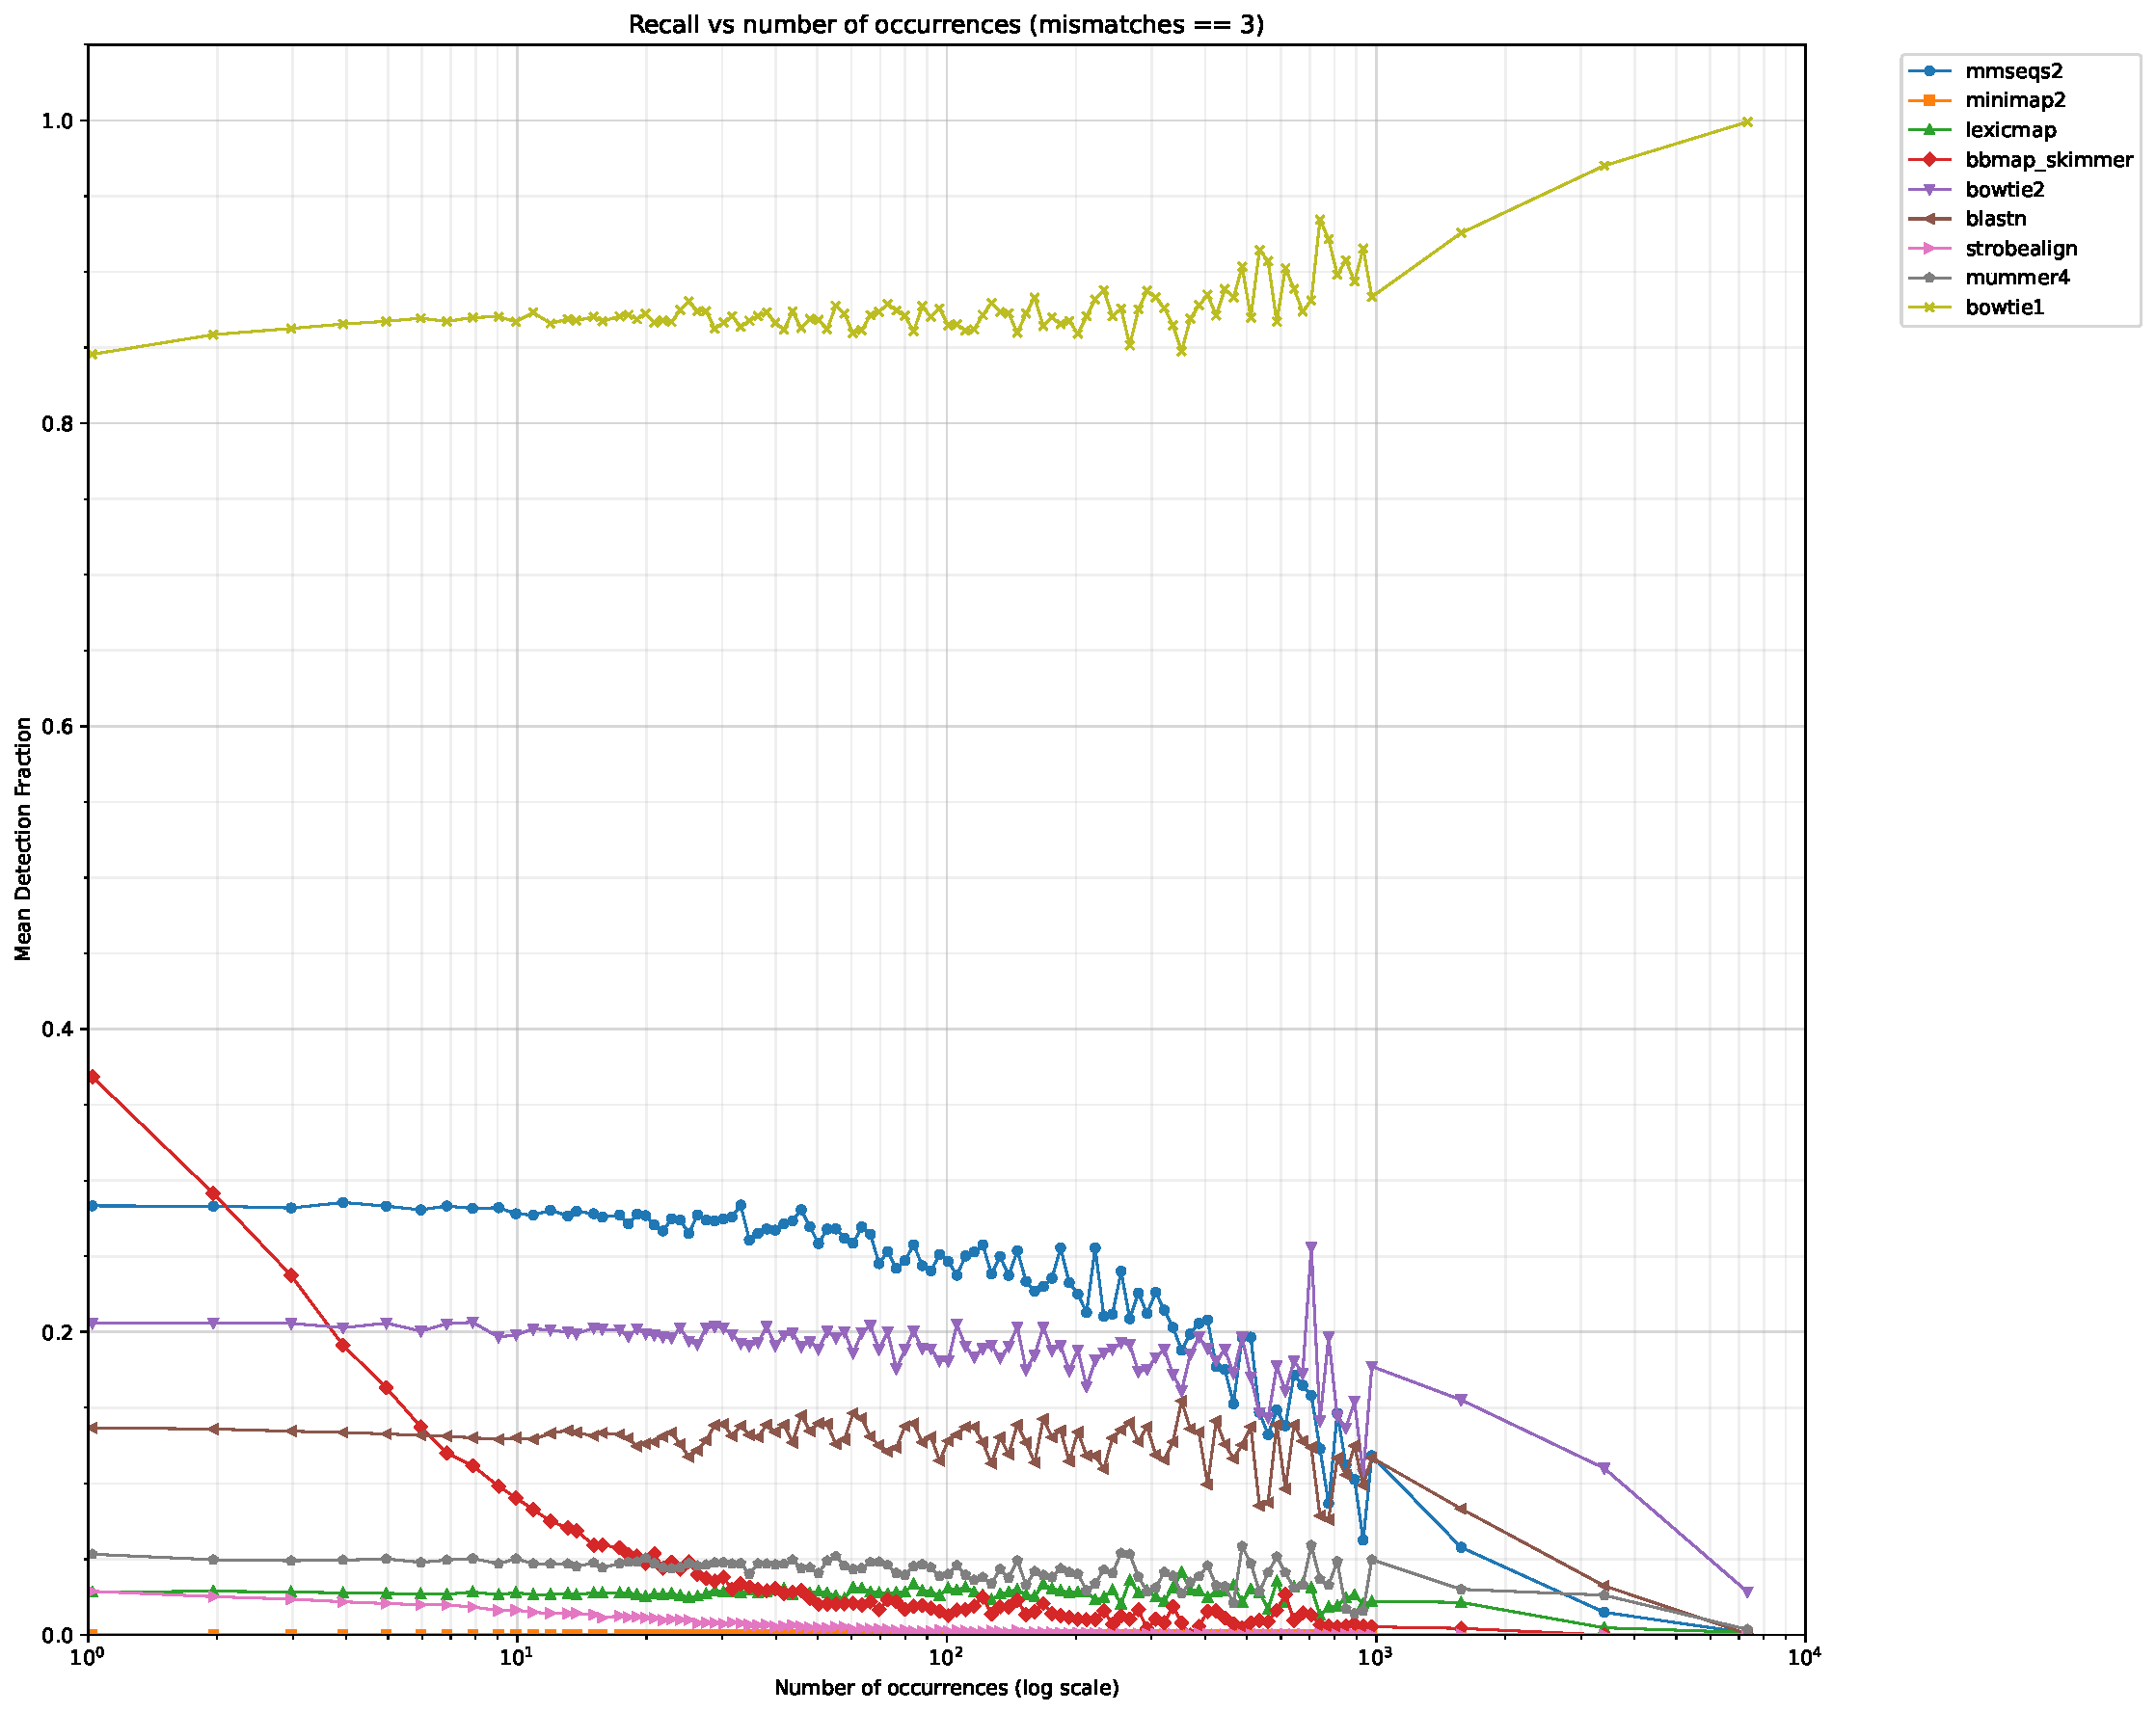
\includegraphics[keepaspectratio]{supplementary_files/mediabag/figures/supp/real_data_recall_vs_occurrences_exact_nm_3.pdf}}

\subsubsection{Supplementary figure 6.}\label{supplementary-figure-6.}

Distributions of spacers characteristics.\\
(A) Spacer size (length in bp)\\
(B) Mismatches observed in spacer alignments\\
(C) Spacer occurrence rate.

\paragraph{1. IMG/VR4 dataset}\label{imgvr4-dataset}

\textbf{Note:} the horizontal axis is logarithmic.

\pandocbounded{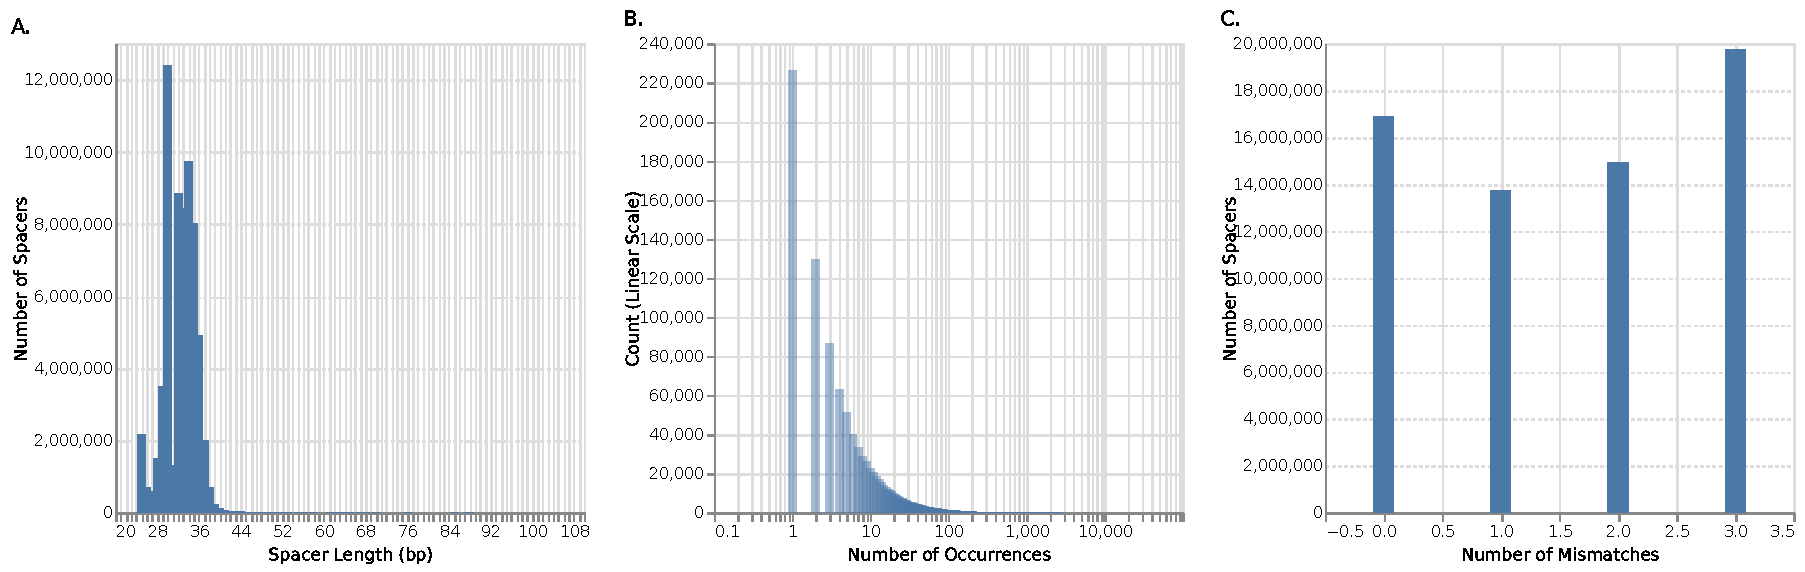
\includegraphics[keepaspectratio]{supplementary_files/mediabag/figures/supp/real_data_spacer_distributions.pdf}}

\paragraph{2. Synthetic dataset}\label{synthetic-dataset}

\pandocbounded{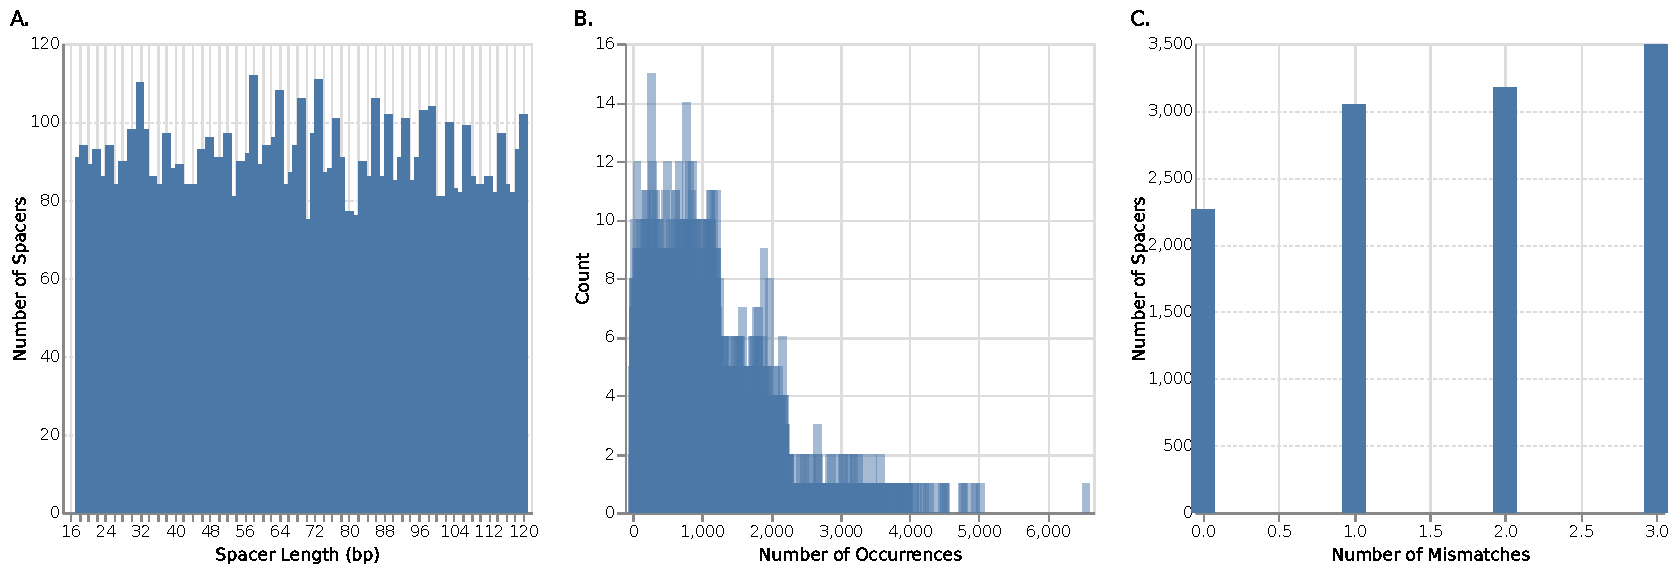
\includegraphics[keepaspectratio]{supplementary_files/mediabag/figures/supp/simulated_spacer_distributions.pdf}}

\subsubsection{Supplementary figure 7.}\label{supplementary-figure-7.}

Upset plot of tool performance for IMG/VR4 dataset. The panels (from top
to bottom) are sorted by number of mismatches. The sets in each panel
are sorted from left to right by the set size. Each row in each panel
represents a tool, and the vertical lines connecting the dots indicate
the intersection of the connected tool results'.

\paragraph{A. 0 mismatches}\label{a.-0-mismatches}

\pandocbounded{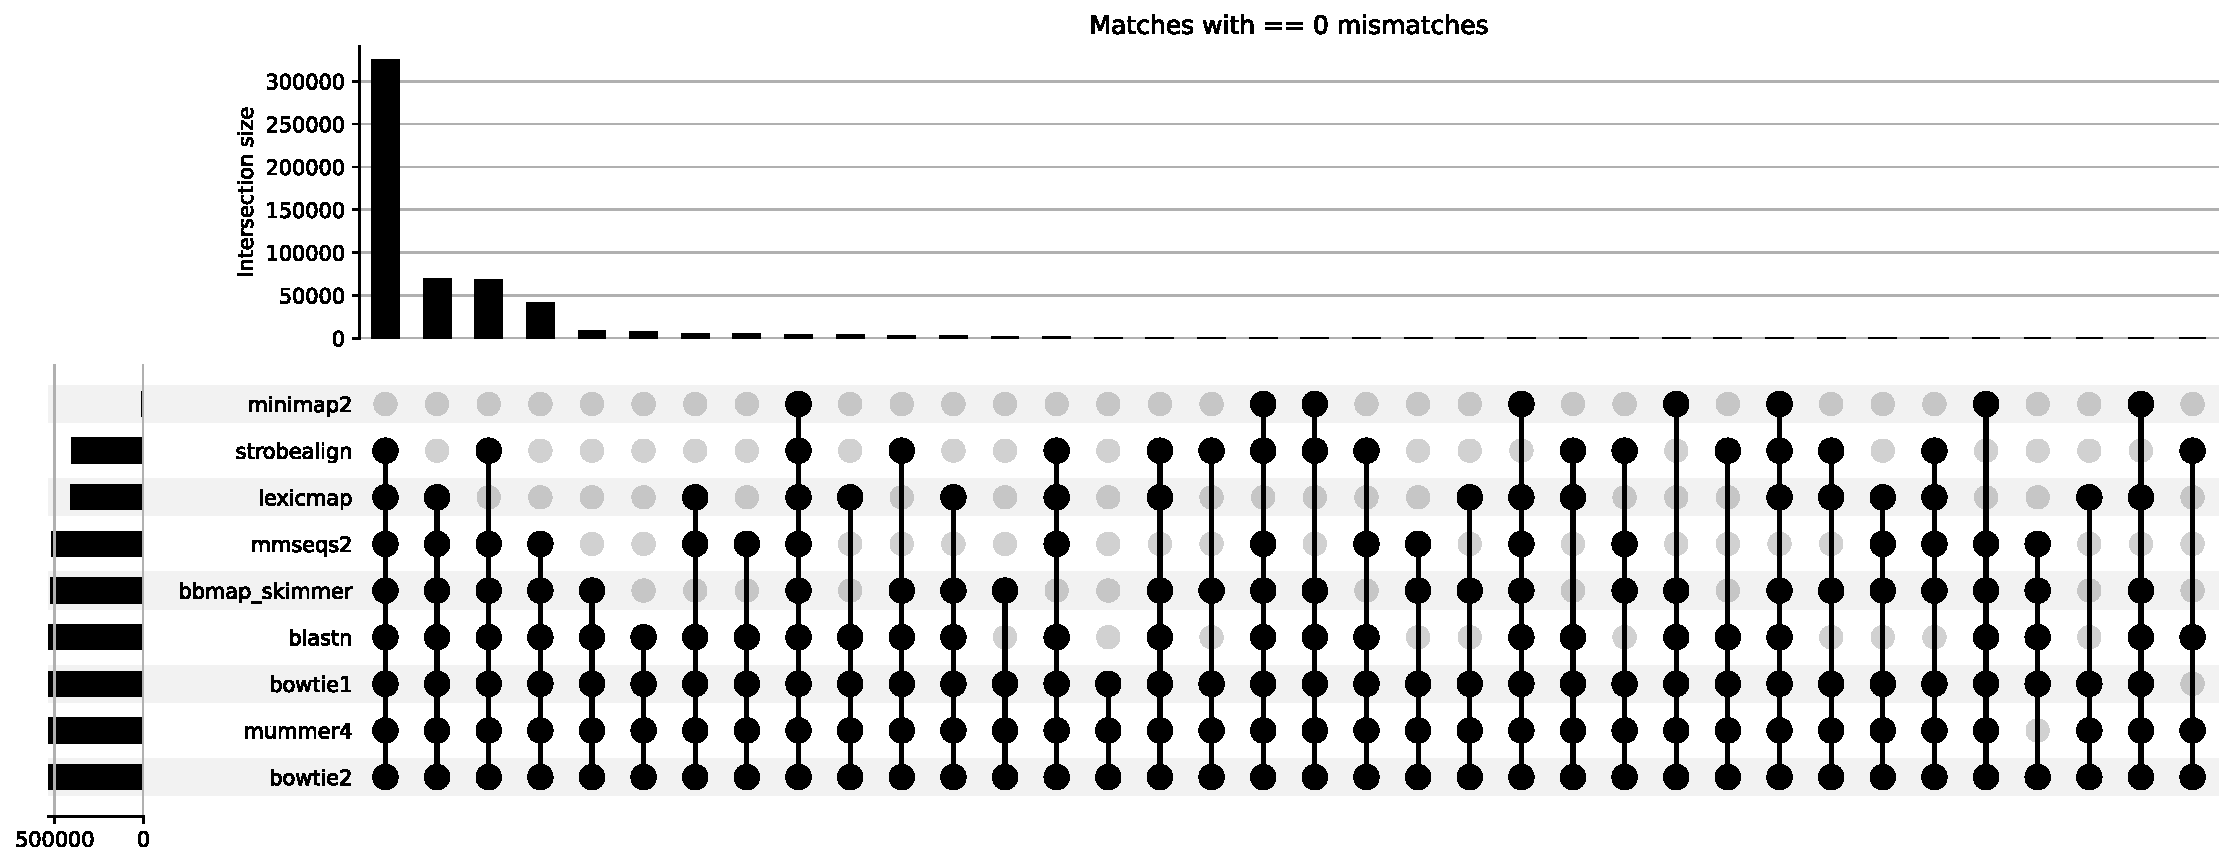
\includegraphics[keepaspectratio]{supplementary_files/mediabag/figures/supp/upset_0.pdf}}

\paragraph{B. 1 mismatch}\label{b.-1-mismatch-1}

\pandocbounded{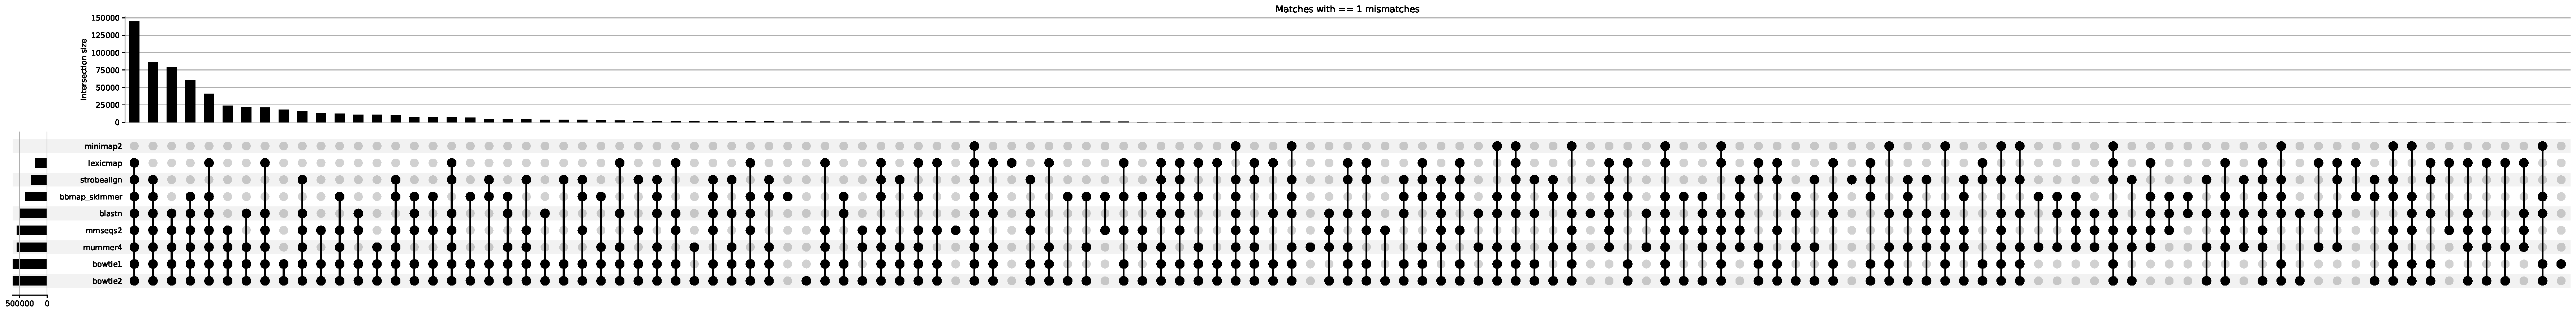
\includegraphics[keepaspectratio]{supplementary_files/mediabag/figures/supp/upset_1.pdf}}

\paragraph{C. 2 mismatches}\label{c.-2-mismatches-1}

\pandocbounded{
\includegraphics[keepaspectratio]{supplementary_files/mediabag/figures/supp/upset_2.pdf}}

\paragraph{D. 3 mismatches}\label{d.-3-mismatches-1}

\pandocbounded{
\includegraphics[keepaspectratio]{supplementary_files/mediabag/figures/supp/upset_3.pdf}}


\printbibliography



\end{document}
